% =====================================================================
%  Chapter 12: Change of Variables in Multiple Integrals
% =====================================================================

\chapter{Change of Variables in Multiple Integrals}
\label{ch:12}

Chapter \ref{ch:11} ended with two scale factors:
\[
    dV=r\,dr\,d\theta\,dz
\]
in cylindrical coordinates, and
\[
    dV=\rho^2\sin\phi\,d\rho\,d\phi\,d\theta
\]
in spherical coordinates.  We found them by drawing tiny coordinate boxes and asking
how large they became in ordinary space.

That method works, but it feels handmade.  Cylinders and spheres are friendly enough
that we can see the geometry.  A general coordinate change will not always be so kind.
We need one rule that finds the scale factor automatically.

The rule is the determinant.

\section{The geometry of substitution}
\label{sec:12.1}

A substitution is a change of language.  In single-variable calculus, we replaced \(x\)
by a new variable \(u\).  In double integrals, we replace \((x,y)\) by new variables
\((u,v)\).  The new variables may straighten a slanted region, unwrap a circular region,
or turn a difficult boundary into a rectangle.

But changing language changes the size of the small pieces.  That is the whole issue.

\subsection{Single-variable substitution remembered}

Start with the one-dimensional story.  Compute
\[
    \int_0^4 \sqrt{x}\,dx.
\]
Let
\[
    x=u^2.
\]
Since \(x\) runs from \(0\) to \(4\), and we choose \(u\ge0\), the new variable runs from
\[
    u=0
    \qquad\text{to}\qquad
    u=2.
\]
Also,
\[
    dx=2u\,du.
\]
So
\[
\begin{aligned}
    \int_0^4 \sqrt{x}\,dx
    &=
    \int_0^2 \sqrt{u^2}\,(2u)\,du\\
    &=
    \int_0^2 2u^2\,du\\
    &=
    2\left[\frac{u^3}{3}\right]_0^2\\
    &=
    \frac{16}{3}.
\end{aligned}
\]

The factor
\[
    2u
\]
did not appear by magic.  It measures how much an interval in \(u\)-space is stretched
when it becomes an interval in \(x\)-space.

Near a particular value \(u\), a small interval of length \(\Delta u\) becomes an interval
of length approximately
\[
    \Delta x\approx \frac{dx}{du}\Delta u.
\]
For
\[
    x=u^2,
\]
this says
\[
    \Delta x\approx 2u\,\Delta u.
\]
Near \(u=2\), a small \(u\)-interval is stretched by about \(4\).  Near \(u=1/10\), it is
stretched by about \(1/5\).

So the one-dimensional substitution rule is really a measurement rule:
\[
\boxed{
    \text{new small length in }x
    =
    \text{stretch factor}\cdot \text{old small length in }u.
}
\]

In symbols,
\[
    dx=\frac{dx}{du}\,du.
\]
For ordinary positive length, the scale factor is
\[
    \left|\frac{dx}{du}\right|.
\]
For oriented integrals, the sign is allowed to stay.  A negative derivative means the
substitution reverses direction.

The same idea will guide us in the plane.  The only difference is that small intervals
become small parallelograms.

\subsection{From small intervals to small parallelograms}

Suppose a square tile in the \((u,v)\)-plane is sent to the \((x,y)\)-plane by
\[
    T(u,v)=(x,y)=(u+2v,\;3u+v).
\]
The point \((0,0)\) goes to
\[
    (0,0).
\]
The unit step in the \(u\)-direction goes to
\[
    T(1,0)-T(0,0)=(1,3).
\]
The unit step in the \(v\)-direction goes to
\[
    T(0,1)-T(0,0)=(2,1).
\]
So the unit square in the \((u,v)\)-plane becomes the parallelogram spanned by
\[
    \mathbf a=(1,3),
    \qquad
    \mathbf b=(2,1).
\]

Its signed area is
\[
    \det[\mathbf a\ \mathbf b]
    =
    \begin{vmatrix}
        1&2\\
        3&1
    \end{vmatrix}
    =
    1\cdot1-3\cdot2
    =
    -5.
\]
The ordinary area is
\[
    5.
\]

\begin{figure}[h]
\centering
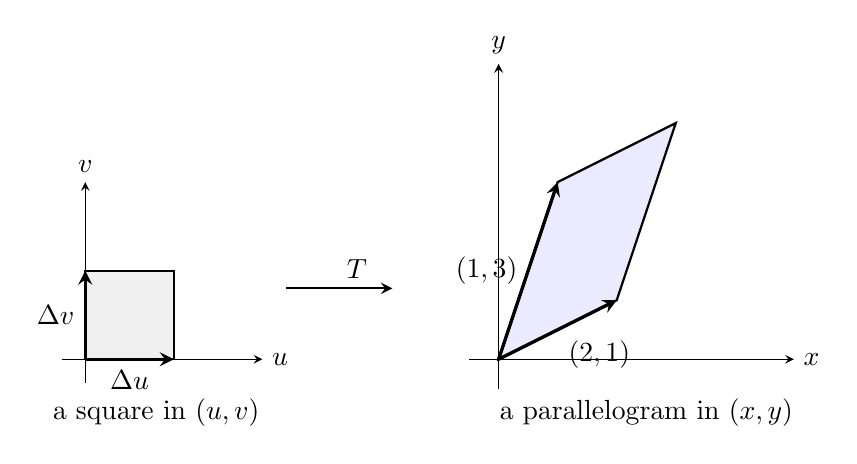
\begin{tikzpicture}[scale=0.75, >=stealth]
    \begin{scope}
        \draw[->] (-0.4,0) -- (3.0,0) node[right] {\(u\)};
        \draw[->] (0,-0.4) -- (0,3.0) node[above] {\(v\)};

        \draw[fill=gray!12, thick] (0,0) rectangle (1.5,1.5);
        \draw[->, very thick] (0,0) -- (1.5,0) node[midway, below] {\(\Delta u\)};
        \draw[->, very thick] (0,0) -- (0,1.5) node[midway, left] {\(\Delta v\)};

        \node at (1.2,-0.9) {a square in \((u,v)\)};
    \end{scope}

    \draw[->, thick] (3.4,1.2) -- (5.2,1.2);
    \node[above] at (4.6,1.2) {\(T\)};

    \begin{scope}[shift={(7,0)}]
        \draw[->] (-0.5,0) -- (5.0,0) node[right] {\(x\)};
        \draw[->] (0,-0.5) -- (0,5.0) node[above] {\(y\)};

        \coordinate (O) at (0,0);
        \coordinate (A) at (1,3);
        \coordinate (B) at (2,1);
        \coordinate (AB) at (3,4);

        \draw[fill=blue!8, thick] (O) -- (A) -- (AB) -- (B) -- cycle;
        \draw[->, very thick] (O) -- (A) node[midway, left] {\((1,3)\)};
        \draw[->, very thick] (O) -- (B) node[midway, below right] {\((2,1)\)};
        \draw[dashed] (A) -- (AB);
        \draw[dashed] (B) -- (AB);

        \node at (2.5,-0.9) {a parallelogram in \((x,y)\)};
    \end{scope}
\end{tikzpicture}
\caption{A linear change of variables sends a square to a parallelogram.  The determinant
measures the signed area of that parallelogram.}
\end{figure}

This is the two-dimensional version of the factor \(dx/du\).  A small square of area
\[
    \Delta u\,\Delta v
\]
is turned into a parallelogram whose area is
\[
    5\,\Delta u\,\Delta v.
\]
The number \(5\) is the area scale factor.

The sign
\[
    -5
\]
also matters.  It says the ordered directions have been flipped.  The \(u\)-direction
followed by the \(v\)-direction becomes a clockwise ordered pair in the \((x,y)\)-plane.
Ordinary area ignores that sign.  Oriented area remembers it.

\subsection{Local linearization of a coordinate map}

The previous map was linear, so every square became a true parallelogram.  Most useful
coordinate maps are not linear.

For example, take
\[
    T(u,v)=(x,y)=(u,\;uv).
\]
This map bends the \((u,v)\)-grid.  A small rectangle in the \((u,v)\)-plane becomes a
curved quadrilateral in the \((x,y)\)-plane.

Still, if the rectangle is tiny, its image is almost a parallelogram.  The two side vectors
come from the partial derivatives of \(T\).

For
\[
    T(u,v)=(x(u,v),y(u,v)),
\]
define
\[
    T_u=(x_u,y_u),
    \qquad
    T_v=(x_v,y_v).
\]
These are the two velocity vectors of the coordinate grid: one obtained by changing
\(u\), the other by changing \(v\).

For
\[
    T(u,v)=(u,uv),
\]
we have
\[
    T_u(u,v)=(1,v),
    \qquad
    T_v(u,v)=(0,u).
\]
At the point
\[
    (u,v)=(2,3),
\]
these become
\[
    T_u(2,3)=(1,3),
    \qquad
    T_v(2,3)=(0,2).
\]
So a tiny rectangle near \((2,3)\), with side lengths \(\Delta u\) and \(\Delta v\), maps
approximately to the parallelogram spanned by
\[
    (1,3)\Delta u
    \qquad\text{and}\qquad
    (0,2)\Delta v.
\]
The signed area scale factor is
\[
    \det
    \begin{pmatrix}
        1&0\\
        3&2
    \end{pmatrix}
    =
    2.
\]
So the image area is approximately
\[
    2\,\Delta u\,\Delta v.
\]

Let us check this with a small actual rectangle:
\[
    2\le u\le2.01,
    \qquad
    3\le v\le3.01.
\]
Since
\[
    x=u,
    \qquad
    y=uv,
\]
the vertical height of the image at a fixed \(u\) is
\[
    u(3.01)-u(3)=0.01u.
\]
Therefore the exact image area is
\[
\begin{aligned}
    \int_{2}^{2.01} 0.01u\,du
    &=
    0.01\left[\frac{u^2}{2}\right]_{2}^{2.01}\\
    &=
    0.01\cdot\frac{2.01^2-2^2}{2}\\
    &=
    0.0002005.
\end{aligned}
\]
The local linear estimate gives
\[
    2(0.01)(0.01)=0.0002.
\]
The agreement is close because the rectangle is small.

\begin{definition}[Jacobian determinant in the plane]
For a differentiable coordinate map
\[
    T(u,v)=(x(u,v),y(u,v)),
\]
the \emph{Jacobian determinant} of \(T\) is
\[
\boxed{
    J_T(u,v)
    =
    \frac{\partial(x,y)}{\partial(u,v)}
    =
    \begin{vmatrix}
        x_u & x_v\\
        y_u & y_v
    \end{vmatrix}
    =
    x_u y_v-x_v y_u.
}
\]
\end{definition}

The notation
\[
    \frac{\partial(x,y)}{\partial(u,v)}
\]
means: the determinant of the derivative matrix of the map from \((u,v)\) to
\((x,y)\).

The geometric meaning is the one we just saw:
\[
\boxed{
    \text{small signed area in }(x,y)
    \approx
    J_T(u,v)\, \text{small signed area in }(u,v).
}
\]
For ordinary area, the local scale factor is
\[
\boxed{
    |J_T(u,v)|.
}
\]

\subsection{Why determinants appear}

The determinant appears because two variables create area, and area is measured by a
two-input object.

The side vectors of a tiny image tile are approximately
\[
    T_u\,du
    \qquad\text{and}\qquad
    T_v\,dv.
\]
The signed area form \(dx\wedge dy\) measures the signed area of those two vectors:
\[
\begin{aligned}
(dx\wedge dy)(T_u,T_v)
&=
\begin{vmatrix}
    x_u & x_v\\
    y_u & y_v
\end{vmatrix}\\
&=
J_T(u,v).
\end{aligned}
\]
So the determinant is not a random correction factor.  It is the signed area of the
parallelogram made by the two coordinate velocity vectors.

The same fact can be written in differential form notation.  Since
\[
    x=x(u,v),
    \qquad
    y=y(u,v),
\]
we have
\[
    dx=x_u\,du+x_v\,dv,
\]
and
\[
    dy=y_u\,du+y_v\,dv.
\]
Then
\[
\begin{aligned}
dx\wedge dy
&=
(x_u\,du+x_v\,dv)\wedge(y_u\,du+y_v\,dv)\\
&=
x_u y_v\,du\wedge dv+x_v y_u\,dv\wedge du\\
&=
(x_u y_v-x_v y_u)\,du\wedge dv.
\end{aligned}
\]
Thus
\[
\boxed{
    dx\wedge dy
    =
    J_T(u,v)\,du\wedge dv.
}
\]
This is the form version of the change in signed area.

There is one condition hidden in the phrase ``local linearization.''  The map must have
a good derivative at the point.  If
\[
    T(u,v)=(|u|,v),
\]
then at the origin the map has a crease.  Approaching from the right, the \(u\)-direction
goes to \((1,0)\).  Approaching from the left, it goes to \((-1,0)\).  There is no single
linear map that describes the behavior from all sides.  So there is no single determinant
at the origin that explains every tiny tile crossing the crease.

Away from the crease, the determinant picture works again.

For a nonlinear coordinate map, the determinant may change from point to point.  That
is why polar coordinates have the factor \(r\), and spherical coordinates have the factor
\(\rho^2\sin\phi\).  Before letting the scale factor vary, it is worth studying the case
where it stays constant.  Linear maps are the cleanest laboratory: every tiny square is
stretched by the same determinant, and the curved-tile approximation becomes exact.

\section{Linear changes of variables}
\label{sec:12.2}

Section \ref{sec:12.1} found the local rule:
\[
    \text{area scale factor}=\left|\frac{\partial(x,y)}{\partial(u,v)}\right|.
\]
For a linear map, this factor is constant.  There is no approximation to manage.  A
square becomes a parallelogram, a rectangle becomes a parallelogram, and every small
piece is scaled by the same amount.

\subsection{Parallelograms from squares}

Let
\[
    T(u,v)=(x,y)=(2u+v,\;u+3v).
\]
The unit square
\[
    0\le u\le1,\qquad 0\le v\le1
\]
has two edge directions:
\[
    \mathbf e_u=(1,0),
    \qquad
    \mathbf e_v=(0,1).
\]
Under \(T\), these become
\[
    T(1,0)-T(0,0)=(2,1),
\]
and
\[
    T(0,1)-T(0,0)=(1,3).
\]
So the unit square becomes the parallelogram spanned by
\[
    \mathbf a=(2,1),
    \qquad
    \mathbf b=(1,3).
\]
Its signed area is
\[
    \det[\mathbf a\ \mathbf b]
    =
    \begin{vmatrix}
        2&1\\
        1&3
    \end{vmatrix}
    =
    6-1
    =
    5.
\]
Thus the ordinary area is \(5\).

The matrix of the map is
\[
    A=
    \begin{pmatrix}
        2&1\\
        1&3
    \end{pmatrix}.
\]
Its determinant is
\[
    \det A=5.
\]
The columns of \(A\) are exactly the images of the two coordinate directions:
\[
    \begin{pmatrix}2\\1\end{pmatrix},
    \qquad
    \begin{pmatrix}1\\3\end{pmatrix}.
\]
So \(\det A\) measures the signed area of the image of the unit square.

\begin{figure}[h]
\centering
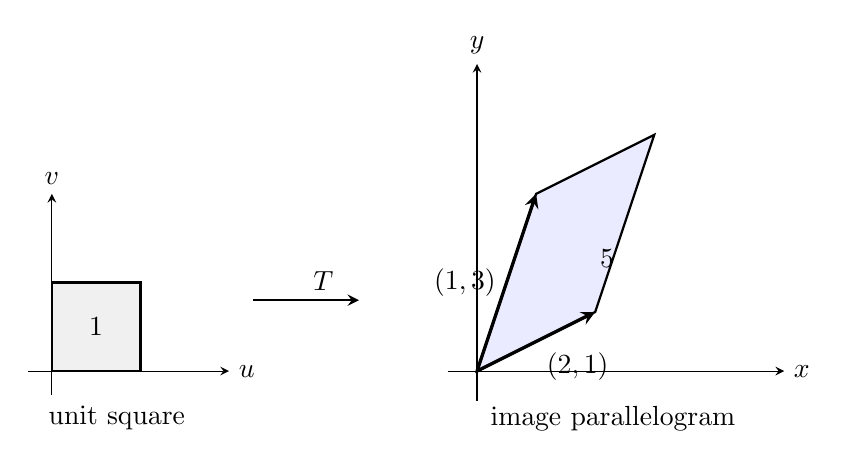
\begin{tikzpicture}[scale=0.75, >=stealth]
    \begin{scope}
        \draw[->] (-0.4,0) -- (3.0,0) node[right] {\(u\)};
        \draw[->] (0,-0.4) -- (0,3.0) node[above] {\(v\)};

        \draw[fill=gray!12, thick] (0,0) rectangle (1.5,1.5);
        \node at (0.75,0.75) {\(1\)};
        \node at (1.1,-0.8) {unit square};
    \end{scope}

    \draw[->, thick] (3.4,1.2) -- (5.2,1.2);
    \node[above] at (4.6,1.2) {\(T\)};

    \begin{scope}[shift={(7.2,0)}]
        \draw[->] (-0.5,0) -- (5.2,0) node[right] {\(x\)};
        \draw[->] (0,-0.5) -- (0,5.2) node[above] {\(y\)};

        \coordinate (O) at (0,0);
        \coordinate (A) at (2,1);
        \coordinate (B) at (1,3);
        \coordinate (AB) at (3,4);

        \draw[fill=blue!8, thick] (O) -- (A) -- (AB) -- (B) -- cycle;
        \draw[->, very thick] (O) -- (A) node[midway, below right] {\((2,1)\)};
        \draw[->, very thick] (O) -- (B) node[midway, left] {\((1,3)\)};
        \draw[dashed] (A) -- (AB);
        \draw[dashed] (B) -- (AB);

        \node at (2.2,1.9) {\(5\)};
        \node at (2.3,-0.8) {image parallelogram};
    \end{scope}
\end{tikzpicture}
\caption{The determinant of a linear map is the signed area of the image of the unit square.}
\end{figure}

If the original square had side length \(0.1\), its area would be \(0.01\), and the image
area would be
\[
    5(0.01)=0.05.
\]
If the original rectangle had area \(7\), the image area would be
\[
    5(7)=35.
\]
A linear map uses the same scale factor everywhere.

\subsection{Area scaling by \texorpdfstring{\(|\det A|\)}{|det A|}}

Now write a general linear change of variables as
\[
    \begin{pmatrix}
    x\\y
    \end{pmatrix}
    =
    A
    \begin{pmatrix}
    u\\v
    \end{pmatrix}
    +
    \mathbf p_0,
\]
where
\[
    A=
    \begin{pmatrix}
        a&b\\
        c&d
    \end{pmatrix}
\]
and \(\mathbf p_0\) is a fixed translation.

The translation moves the region.  It does not change its area.  The matrix \(A\) does
the stretching, shearing, rotating, reflecting, or collapsing.

The coordinate directions become
\[
    \mathbf a=(a,c),
    \qquad
    \mathbf b=(b,d).
\]
The signed area of the parallelogram spanned by them is
\[
    \det A=ad-bc.
\]
So the ordinary area scale factor is
\[
    |\det A|.
\]

\begin{theorem}[Area scaling by a linear map]
Let
\[
    T(\mathbf u)=A\mathbf u+\mathbf p_0
\]
be a linear change followed by a translation, where \(A\) is a \(2\times2\) matrix with
\[
    \det A\ne0.
\]
If \(S\) is a region in the \((u,v)\)-plane and
\[
    R=T(S)
\]
is its image in the \((x,y)\)-plane, then
\[
\boxed{
    \operatorname{Area}(R)=|\det A|\,\operatorname{Area}(S).
}
\]
More generally, for any function \(f\) for which the integrals exist,
\[
\boxed{
    \iint_R f(x,y)\,dA
    =
    \iint_S f(T(u,v))\,|\det A|\,du\,dv.
}
\]
\end{theorem}

\begin{proof}
Cut \(S\) into many small rectangles.  A rectangle with side lengths
\[
    \Delta u,\qquad \Delta v
\]
has area
\[
    \Delta u\,\Delta v.
\]
The map \(T\) sends its side directions to
\[
    \mathbf a\,\Delta u
    \qquad\text{and}\qquad
    \mathbf b\,\Delta v.
\]
The image is a parallelogram with ordinary area
\[
    |\det[\mathbf a\ \mathbf b]|\,\Delta u\,\Delta v
    =
    |\det A|\,\Delta u\,\Delta v.
\]
Adding these image pieces gives the area formula.

For the integral formula, the contribution from one small image piece is approximately
\[
    f(T(u^*,v^*))\,|\det A|\,\Delta u\,\Delta v.
\]
Adding all pieces and passing to the integral gives
\[
    \iint_R f(x,y)\,dA
    =
    \iint_S f(T(u,v))\,|\det A|\,du\,dv.
\]
\end{proof}

The condition
\[
    \det A\ne0
\]
is the condition that the map does not collapse the plane.

Here is what breaks without it.  Let
\[
    A=
    \begin{pmatrix}
        1&1\\
        2&2
    \end{pmatrix}.
\]
Then
\[
    T(u,v)=(u+v,\;2u+2v).
\]
The unit square in the \((u,v)\)-plane does not become a two-dimensional region.  It
collapses onto the line segment
\[
    y=2x,
    \qquad
    0\le x\le2.
\]
The determinant is
\[
    \det A=1\cdot2-1\cdot2=0.
\]
A two-dimensional area has been crushed to area \(0\).  This is not a valid
two-dimensional change of variables for a double integral over a region with area.

\subsection{Orientation and the sign of the determinant}

Ordinary area uses
\[
    |\det A|.
\]
Oriented area uses
\[
    \det A.
\]

The simplest example is reflection across the \(x\)-axis:
\[
    T(u,v)=(u,-v).
\]
Here
\[
    A=
    \begin{pmatrix}
        1&0\\
        0&-1
    \end{pmatrix},
    \qquad
    \det A=-1.
\]
The unit square still has ordinary area \(1\).  Its image still has ordinary area \(1\).
But the orientation has reversed.

The ordered pair
\[
    \mathbf e_u,\mathbf e_v
\]
turns counterclockwise in the \((u,v)\)-plane.  Its image is
\[
    (1,0),(0,-1),
\]
which turns clockwise in the \((x,y)\)-plane.  That is why the signed area scale factor
is \(-1\).

In form language, this sign is automatic.  If
\[
    x=au+bv,
    \qquad
    y=cu+dv,
\]
then
\[
    dx=a\,du+b\,dv,
\]
and
\[
    dy=c\,du+d\,dv.
\]
Therefore
\[
\begin{aligned}
dx\wedge dy
&=
(a\,du+b\,dv)\wedge(c\,du+d\,dv)\\
&=
(ad-bc)\,du\wedge dv\\
&=
(\det A)\,du\wedge dv.
\end{aligned}
\]
So
\[
\boxed{
    dx\wedge dy=(\det A)\,du\wedge dv.
}
\]

This is the oriented change-of-variables rule.  The ordinary area rule takes absolute
value:
\[
\boxed{
    dA=|\det A|\,du\,dv.
}
\]

The sign is not an inconvenience.  It carries information.  Later, when we integrate
forms over oriented curves and surfaces, this sign will become the reason boundary
orientation works cleanly.

\subsection{Examples with rotated and skewed regions}

A linear change of variables is useful when the region is a parallelogram, a rotated
rectangle, or any shape whose boundaries become simpler after a linear transformation.

\begin{example}[A density over a skewed floor tile]
Let \(R\) be the parallelogram spanned by
\[
    (2,1)
    \qquad\text{and}\qquad
    (1,3),
\]
starting at the origin.  Find
\[
    \iint_R (x+y)\,dA.
\]

Use the square
\[
    S=\{(u,v):0\le u\le1,\ 0\le v\le1\}
\]
and the map
\[
    x=2u+v,
    \qquad
    y=u+3v.
\]
Then
\[
    A=
    \begin{pmatrix}
        2&1\\
        1&3
    \end{pmatrix},
    \qquad
    |\det A|=5.
\]
Also,
\[
    x+y=(2u+v)+(u+3v)=3u+4v.
\]
Therefore
\[
\begin{aligned}
\iint_R (x+y)\,dA
&=
\int_0^1\int_0^1 (3u+4v)\,5\,dv\,du\\
&=
5\int_0^1\left[3uv+2v^2\right]_{0}^{1}\,du\\
&=
5\int_0^1(3u+2)\,du\\
&=
5\left(\frac32+2\right)\\
&=
\frac{35}{2}.
\end{aligned}
\]
So
\[
\boxed{
    \iint_R (x+y)\,dA=\frac{35}{2}.
}
\]
The parallelogram became a square, and the determinant supplied the area correction.
\end{example}

\begin{example}[A rotated rectangle]
A rectangle has been rotated by \(45^\circ\).  Instead of describing its slanted sides in
\(x\) and \(y\), use coordinates \(u\) and \(v\) along the rotated axes:
\[
    x=\frac{u-v}{\sqrt2},
    \qquad
    y=\frac{u+v}{\sqrt2}.
\]
This is a rotation, so it should preserve area.  The determinant confirms it:
\[
    A=
    \begin{pmatrix}
        1/\sqrt2 & -1/\sqrt2\\
        1/\sqrt2 & 1/\sqrt2
    \end{pmatrix},
\]
and
\[
    \det A
    =
    \frac12+\frac12
    =
    1.
\]

Let \(R\) be the image of
\[
    0\le u\le3,
    \qquad
    0\le v\le1.
\]
Compute
\[
    \iint_R (x^2+y^2)\,dA.
\]
Under the rotation,
\[
\begin{aligned}
x^2+y^2
&=
\left(\frac{u-v}{\sqrt2}\right)^2
+
\left(\frac{u+v}{\sqrt2}\right)^2\\
&=
u^2+v^2.
\end{aligned}
\]
Since \(|\det A|=1\),
\[
\begin{aligned}
\iint_R (x^2+y^2)\,dA
&=
\int_0^3\int_0^1 (u^2+v^2)\,dv\,du\\
&=
\int_0^3\left(u^2+\frac13\right)\,du\\
&=
9+1\\
&=
10.
\end{aligned}
\]
So
\[
\boxed{
    \iint_R (x^2+y^2)\,dA=10.
}
\]
The region was slanted in \(x,y\), but rectangular in \(u,v\).
\end{example}

Linear maps are now under control.  Their scale factor is constant because their grid
lines stay straight and evenly spaced.  But polar coordinates do not behave that way.
Near the origin, angular wedges are tiny; far from the origin, the same angle covers a
long arc.  The determinant must change from point to point.  The next step is to let the
matrix of partial derivatives vary across the region and to trust the same local
parallelogram idea everywhere at once.
\section{Nonlinear changes of variables in the plane}
\label{sec:12.3}

Section \ref{sec:12.2} treated linear changes of variables.  A square became a
parallelogram, and one number,
\[
    |\det A|,
\]
scaled every area in the same way.

Now the grid is allowed to bend.  A small square may become a small curved tile.  But
if the square is tiny, the curved tile is almost a parallelogram, and the determinant
still measures its area.  The only difference is that the determinant may change from
point to point.

\subsection{The change-of-variables theorem in two dimensions}

Start with a map that is nonlinear, but still easy to see:
\[
    T(u,v)=(x,y)=(u,uv).
\]
Let
\[
    S=\{(u,v):1\le u\le3,\ 0\le v\le2\}.
\]
Since
\[
    x=u,\qquad y=uv,
\]
the image region \(R=T(S)\) satisfies
\[
    1\le x\le3,
    \qquad
    0\le y\le 2x.
\]
So a rectangle in the \((u,v)\)-plane becomes a wedge-shaped region in the
\((x,y)\)-plane.

\begin{figure}[h]
\centering
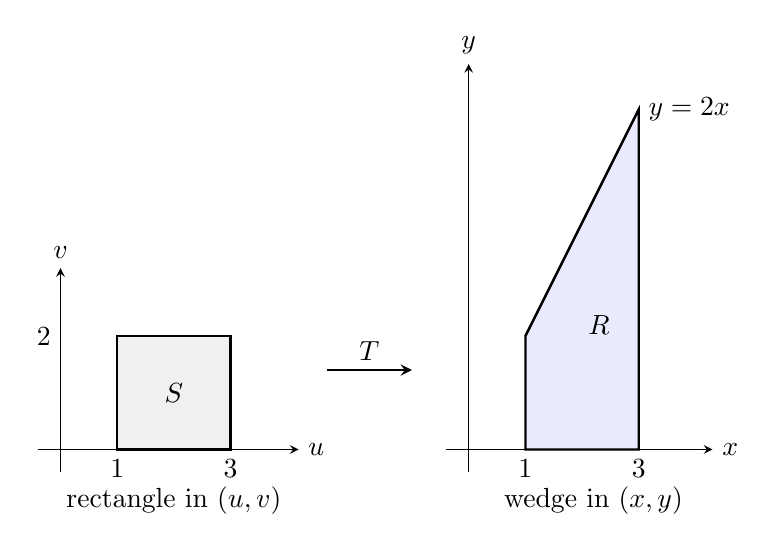
\begin{tikzpicture}[scale=0.72, >=stealth]
    \begin{scope}
        \draw[->] (-0.4,0) -- (4.2,0) node[right] {\(u\)};
        \draw[->] (0,-0.4) -- (0,3.2) node[above] {\(v\)};

        \draw[fill=gray!12, thick] (1,0) rectangle (3,2);
        \node[below] at (1,0) {\(1\)};
        \node[below] at (3,0) {\(3\)};
        \node[left] at (0,2) {\(2\)};
        \node at (2,1) {\(S\)};
        \node at (2,-0.9) {rectangle in \((u,v)\)};
    \end{scope}

    \draw[->, thick] (4.7,1.4) -- (6.2,1.4);
    \node[above] at (5.45,1.4) {\(T\)};

    \begin{scope}[shift={(7.2,0)}]
        \draw[->] (-0.4,0) -- (4.3,0) node[right] {\(x\)};
        \draw[->] (0,-0.4) -- (0,6.8) node[above] {\(y\)};

        \draw[fill=blue!8, thick] (1,0) -- (3,0) -- (3,6) -- (1,2) -- cycle;

        \draw[dashed] (1,0) -- (1,2);
        \draw[dashed] (3,0) -- (3,6);
        \draw[thick] (1,2) -- (3,6);

        \node[below] at (1,0) {\(1\)};
        \node[below] at (3,0) {\(3\)};
        \node[right] at (3,6) {\(y=2x\)};
        \node at (2.3,2.2) {\(R\)};
        \node at (2.2,-0.9) {wedge in \((x,y)\)};
    \end{scope}
\end{tikzpicture}
\caption{The nonlinear map \(T(u,v)=(u,uv)\) sends a rectangle to a wedge.}
\end{figure}

Let us find the area of \(R\) in two ways.

In \(x,y\)-coordinates, the region is
\[
    1\le x\le3,\qquad 0\le y\le2x.
\]
So
\[
\begin{aligned}
    \operatorname{Area}(R)
    &=
    \int_1^3\int_0^{2x}1\,dy\,dx\\
    &=
    \int_1^3 2x\,dx\\
    &=
    \left[x^2\right]_1^3\\
    &=
    8.
\end{aligned}
\]

Now compute the same area from the rectangle \(S\).  The derivative vectors of the map
are
\[
    T_u=(1,v),
    \qquad
    T_v=(0,u).
\]
The signed area scale factor is
\[
    J_T(u,v)
    =
    \det
    \begin{pmatrix}
        1&0\\
        v&u
    \end{pmatrix}
    =
    u.
\]
Since \(u\ge1\) on \(S\), the ordinary area scale factor is
\[
    |J_T(u,v)|=u.
\]
Therefore
\[
\begin{aligned}
    \operatorname{Area}(R)
    &=
    \int_1^3\int_0^2 u\,dv\,du\\
    &=
    \int_1^3 2u\,du\\
    &=
    8.
\end{aligned}
\]

The computation says something geometric.  The vertical \(v\)-direction is stretched
by the factor \(u\).  When \(u=1\), a small \(v\)-step has length about \(1\).  When
\(u=3\), the same \(v\)-step has length about \(3\).  The grid spreads out as \(u\)
increases.

The determinant is no longer one constant number.  It is a function:
\[
    J_T(u,v)=u.
\]

\begin{definition}[Jacobian determinant in the plane]
For a differentiable map
\[
    T(u,v)=(x(u,v),y(u,v)),
\]
the \emph{Jacobian determinant} is
\[
\boxed{
    J_T(u,v)
    =
    \frac{\partial(x,y)}{\partial(u,v)}
    =
    \det
    \begin{pmatrix}
        x_u & x_v\\
        y_u & y_v
    \end{pmatrix}
    =
    x_u y_v-x_v y_u.
}
\]
The ordinary local area scale factor is
\[
\boxed{
    |J_T(u,v)|.
}
\]
\end{definition}

The change-of-variables theorem says that this local scale factor can be added over
the whole region.

\begin{theorem}[Change of variables in the plane]
Let \(S\) be a bounded region in the \((u,v)\)-plane, and let
\[
    T(u,v)=(x(u,v),y(u,v))
\]
be a coordinate map from \(S\) to a region \(R\) in the \((x,y)\)-plane.

Assume:

\begin{enumerate}
\item \(T\) has continuous first partial derivatives on a region containing \(S\);

\item \(T\) is one-to-one on the interior of \(S\), except possibly along boundary
pieces;

\item \(J_T(u,v)\ne0\) on the interior of \(S\).
\end{enumerate}

If \(f\) is continuous on \(R=T(S)\), then
\[
\boxed{
    \iint_R f(x,y)\,dA
    =
    \iint_S f(x(u,v),y(u,v))\,|J_T(u,v)|\,du\,dv.
}
\]
\end{theorem}

\begin{proof}[Proof idea]
Cut \(S\) into many tiny rectangles.  Near a point \((u,v)\), the map \(T\) is well
approximated by its derivative:
\[
    T(u+\Delta u,v+\Delta v)
    \approx
    T(u,v)+T_u\,\Delta u+T_v\,\Delta v.
\]
So a tiny rectangle in the \((u,v)\)-plane maps almost to a parallelogram spanned by
\[
    T_u\,\Delta u
    \qquad\text{and}\qquad
    T_v\,\Delta v.
\]
The area of that parallelogram is approximately
\[
    |J_T(u,v)|\,\Delta u\,\Delta v.
\]
Thus a small contribution in the image is approximately
\[
    f(T(u,v))\,|J_T(u,v)|\,\Delta u\,\Delta v.
\]
Adding all pieces and letting the rectangles shrink gives the formula.
\end{proof}

The theorem has hypotheses because the determinant is a local story.  It measures how
one tiny tile is stretched near one point.  A global change of variables must also avoid
overlapping the same image region more than once.

\subsection{The Jacobian determinant}

The map
\[
    T(u,v)=(u,uv)
\]
was chosen because the geometry was visible.  Now use the theorem on a real integral.

Let \(R\) be the wedge
\[
    1\le x\le3,\qquad 0\le y\le2x.
\]
Compute
\[
    \iint_R (x+y)\,dA.
\]
Use
\[
    x=u,\qquad y=uv,
\]
with
\[
    1\le u\le3,\qquad 0\le v\le2.
\]
The Jacobian determinant is
\[
    J_T(u,v)=u.
\]
Also,
\[
    x+y=u+uv=u(1+v).
\]
Therefore
\[
\begin{aligned}
    \iint_R (x+y)\,dA
    &=
    \int_1^3\int_0^2 u(1+v)\,u\,dv\,du\\
    &=
    \int_1^3 u^2
    \left[\int_0^2(1+v)\,dv\right]du\\
    &=
    \int_1^3 u^2
    \left[v+\frac{v^2}{2}\right]_0^2du\\
    &=
    \int_1^3 4u^2\,du\\
    &=
    4\left[\frac{u^3}{3}\right]_1^3\\
    &=
    \frac{104}{3}.
\end{aligned}
\]
So
\[
\boxed{
    \iint_R (x+y)\,dA=\frac{104}{3}.
}
\]

Notice the two substitutions that happened at once:
\[
    x+y
    \quad\longrightarrow\quad
    u+uv,
\]
and
\[
    dA
    \quad\longrightarrow\quad
    u\,du\,dv.
\]
The first substitution changes the function.  The second changes the tiny area piece.

In differential form language, the signed area element changes by
\[
\boxed{
    dx\wedge dy
    =
    J_T(u,v)\,du\wedge dv.
}
\]
For ordinary area integrals, we use the absolute value:
\[
\boxed{
    dA=|J_T(u,v)|\,du\,dv.
}
\]

\subsection{One-to-one conditions and splitting regions}

The one-to-one condition is easy to underestimate.  A determinant can measure the
right local scale and still give the wrong global answer if the map covers the same
region twice.

Consider
\[
    T(u,v)=(u^2,v)
\]
on the rectangle
\[
    S=[-1,1]\times[0,1].
\]
The image is the unit square
\[
    R=[0,1]\times[0,1].
\]
The Jacobian determinant is
\[
    J_T(u,v)
    =
    \det
    \begin{pmatrix}
        2u&0\\
        0&1
    \end{pmatrix}
    =
    2u.
\]
If we blindly integrate the area scale factor over all of \(S\), we get
\[
\begin{aligned}
    \iint_S |2u|\,du\,dv
    &=
    \int_0^1\int_{-1}^1 |2u|\,du\,dv\\
    &=
    2.
\end{aligned}
\]
But the image square has area
\[
    1.
\]
The formula counted most of the image twice: once from \(u>0\), and once from
\(u<0\).

The fix is not to throw away the Jacobian.  The fix is to choose a one-to-one branch.
For example, on
\[
    0\le u\le1,\qquad 0\le v\le1,
\]
the same map covers the unit square once, and
\[
\begin{aligned}
    \iint_{[0,1]\times[0,1]} 2u\,du\,dv
    &=
    1.
\end{aligned}
\]
The determinant was right locally.  The region was wrong globally.

A second warning is smoothness.  Take
\[
    T(u,v)=(u,\ v+|u|).
\]
This map is one-to-one, but it has a crease along
\[
    u=0.
\]
On the right side, where \(u>0\),
\[
    T(u,v)=(u,v+u).
\]
On the left side, where \(u<0\),
\[
    T(u,v)=(u,v-u).
\]
The derivative changes suddenly across the crease.  There is no single linear map that
describes \(T\) at points with \(u=0\).

A tile crossing the crease does not have one clean tangent parallelogram.  To use the
change-of-variables theorem, split the domain into two pieces:
\[
    u\ge0
    \qquad\text{and}\qquad
    u\le0.
\]
Each piece is smooth.  Then compute on the pieces separately.

The nonzero-Jacobian condition also has a geometric meaning.  If
\[
    J_T=0
\]
throughout a patch, then tiny area can be crushed to zero area.  For example,
\[
    T(u,v)=(u,0)
\]
sends the whole unit square onto a line segment.  Its Jacobian determinant is
\[
    0,
\]
and the image has no two-dimensional area.

A zero Jacobian at a boundary point is often harmless.  Polar coordinates have
\[
    J=r,
\]
which vanishes at \(r=0\).  That single point does not ruin the area formula.  But a
coordinate change should not collapse a whole two-dimensional piece if we want it to
describe a two-dimensional region.

\subsection{Polar coordinates revisited as a theorem, not a trick}

Polar coordinates are the most familiar nonlinear change of variables:
\[
    x=r\cos\theta,
    \qquad
    y=r\sin\theta.
\]
Before, the factor
\[
    r
\]
came from the length of a circular arc:
\[
    \text{arc length}\approx r\,\Delta\theta.
\]
Now the same factor comes automatically from the Jacobian determinant.

Compute:
\[
    x_r=\cos\theta,
    \qquad
    x_\theta=-r\sin\theta,
\]
and
\[
    y_r=\sin\theta,
    \qquad
    y_\theta=r\cos\theta.
\]
Therefore
\[
\begin{aligned}
    \frac{\partial(x,y)}{\partial(r,\theta)}
    &=
    \det
    \begin{pmatrix}
        \cos\theta & -r\sin\theta\\
        \sin\theta & r\cos\theta
    \end{pmatrix}\\
    &=
    r\cos^2\theta+r\sin^2\theta\\
    &=
    r.
\end{aligned}
\]
So
\[
\boxed{
    dA=r\,dr\,d\theta.
}
\]

This is the old polar area element, now explained by the same determinant rule used
for every coordinate change.

\begin{example}[Dye in a circular spill]
A circular spill occupies the disk
\[
    x^2+y^2\le4.
\]
The dye concentration at \((x,y)\) is
\[
    q(x,y)=12-x^2-y^2.
\]
Find the total amount of dye.

In polar coordinates,
\[
    x^2+y^2=r^2,
\]
so
\[
    q=12-r^2.
\]
The disk is
\[
    0\le r\le2,\qquad 0\le\theta\le2\pi.
\]
Therefore
\[
\begin{aligned}
    Q
    &=
    \iint_R (12-x^2-y^2)\,dA\\
    &=
    \int_0^{2\pi}\int_0^2 (12-r^2)\,r\,dr\,d\theta\\
    &=
    2\pi\int_0^2(12r-r^3)\,dr\\
    &=
    2\pi
    \left[
        6r^2-\frac{r^4}{4}
    \right]_0^2\\
    &=
    2\pi(24-4)\\
    &=
    40\pi.
\end{aligned}
\]
So
\[
\boxed{
    Q=40\pi.
}
\]
\end{example}

Polar coordinates are nearly one-to-one on the usual rectangle
\[
    0\le r\le a,\qquad 0\le\theta\le2\pi.
\]
The only overlaps occur on the boundary:
\[
    \theta=0
    \qquad\text{and}\qquad
    \theta=2\pi,
\]
and all points with \(r=0\) become the origin.  These boundary overlaps do not change
the integral.

But if we use
\[
    0\le\theta\le4\pi,
\]
then the disk is traced twice.  The integral will be twice as large unless we intend to
count multiplicity.  This is the same one-to-one warning in a familiar disguise.

The plane story is now complete enough to trust.  A nonlinear map bends a grid, but
each tiny tile is still governed by a determinant.  In space, the same idea has one more
edge: tiny boxes become tiny parallelepipeds, and the determinant becomes a
\(3\times3\) volume scale factor.

\section{Changes of variables in space}
\label{sec:12.4}

Section \ref{sec:12.3} turned a tiny square into a tiny parallelogram.  The area scale
factor was the absolute value of a \(2\times2\) determinant.

A spatial coordinate change turns a tiny box into a tiny parallelepiped.  The volume
scale factor is the absolute value of a \(3\times3\) determinant.

\subsection{Volume scaling by the Jacobian determinant}

Begin with a transformation that turns a box into a solid with a curved ceiling:
\[
    T(u,v,w)=(x,y,z)=(u,\ v,\ uvw).
\]
Let
\[
    S=\{(u,v,w):1\le u\le2,\ 1\le v\le3,\ 0\le w\le1\}.
\]
Since
\[
    x=u,\qquad y=v,\qquad z=uvw,
\]
the image \(E=T(S)\) is
\[
    1\le x\le2,
    \qquad
    1\le y\le3,
    \qquad
    0\le z\le xy.
\]
So the simple box in \(u,v,w\)-coordinates becomes the solid under the surface
\[
    z=xy
\]
over the rectangle \(1\le x\le2,\ 1\le y\le3\).

Compute the volume directly:
\[
\begin{aligned}
    \operatorname{Vol}(E)
    &=
    \int_1^2\int_1^3\int_0^{xy}1\,dz\,dy\,dx\\
    &=
    \int_1^2\int_1^3 xy\,dy\,dx\\
    &=
    \left[\int_1^2 x\,dx\right]
    \left[\int_1^3 y\,dy\right]\\
    &=
    \frac32\cdot4\\
    &=
    6.
\end{aligned}
\]

Now compute the same volume by the transformation.

The derivative matrix is
\[
    DT(u,v,w)
    =
    \begin{pmatrix}
        x_u&x_v&x_w\\
        y_u&y_v&y_w\\
        z_u&z_v&z_w
    \end{pmatrix}
    =
    \begin{pmatrix}
        1&0&0\\
        0&1&0\\
        vw&uw&uv
    \end{pmatrix}.
\]
Its determinant is
\[
    J_T(u,v,w)=uv.
\]
Therefore
\[
\begin{aligned}
    \operatorname{Vol}(E)
    &=
    \int_1^2\int_1^3\int_0^1 uv\,dw\,dv\,du\\
    &=
    \left[\int_1^2 u\,du\right]
    \left[\int_1^3 v\,dv\right]
    \left[\int_0^1 1\,dw\right]\\
    &=
    \frac32\cdot4\cdot1\\
    &=
    6.
\end{aligned}
\]

Again the determinant is the scale factor.  Here \(w\) measures the fraction of the way
from the floor \(z=0\) to the ceiling \(z=xy\).  A small \(w\)-step corresponds to a
vertical \(z\)-step of length approximately
\[
    xy\,\Delta w=uv\,\Delta w.
\]
That is why the factor is \(uv\).

\begin{figure}[h]
\centering
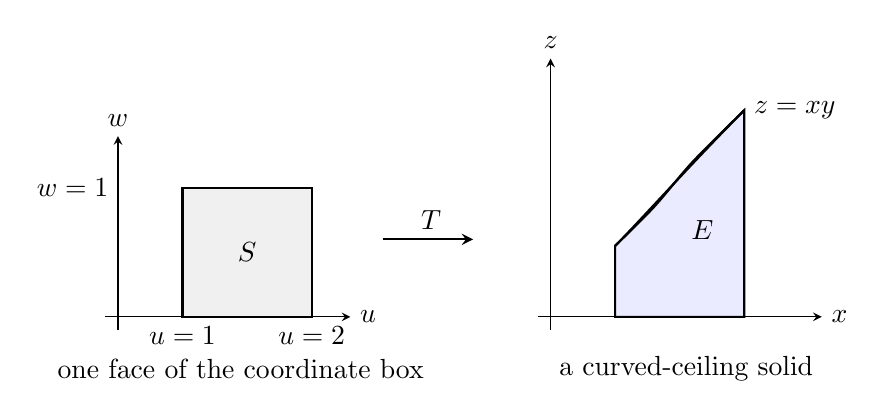
\begin{tikzpicture}[scale=0.82, >=stealth]
    \begin{scope}
        \draw[->] (-0.2,0) -- (3.6,0) node[right] {\(u\)};
        \draw[->] (0,-0.2) -- (0,2.8) node[above] {\(w\)};

        \draw[fill=gray!12, thick] (1,0) rectangle (3,2);
        \node at (2,1) {\(S\)};
        \node[below] at (1,0) {\(u=1\)};
        \node[below] at (3,0) {\(u=2\)};
        \node[left] at (0,2) {\(w=1\)};
        \node at (1.9,-0.8) {one face of the coordinate box};
    \end{scope}

    \draw[->, thick] (4.1,1.2) -- (5.5,1.2);
    \node[above] at (4.85,1.2) {\(T\)};

    \begin{scope}[shift={(6.7,0)}]
        \draw[->] (-0.2,0) -- (4.2,0) node[right] {\(x\)};
        \draw[->] (0,-0.2) -- (0,4.0) node[above] {\(z\)};

        \draw[thick, fill=blue!8]
            (1,0) -- (3,0) -- (3,3.2)
            .. controls (2.2,2.4) and (1.4,1.5) ..
            (1,1.1) -- cycle;

        \draw[thick]
            plot[smooth] coordinates {(1,1.1) (1.6,1.7) (2.2,2.4) (3,3.2)};
        \node at (2.35,1.35) {\(E\)};
        \node[right] at (3,3.2) {\(z=xy\)};
        \node at (2.1,-0.8) {a curved-ceiling solid};
    \end{scope}
\end{tikzpicture}
\caption{A simple coordinate box can become a solid whose height depends on position.}
\end{figure}

\begin{definition}[Jacobian determinant in space]
For a differentiable map
\[
    T(u,v,w)=(x(u,v,w),y(u,v,w),z(u,v,w)),
\]
the \emph{Jacobian determinant} is
\[
\boxed{
    J_T(u,v,w)
    =
    \frac{\partial(x,y,z)}{\partial(u,v,w)}
    =
    \det
    \begin{pmatrix}
        x_u&x_v&x_w\\
        y_u&y_v&y_w\\
        z_u&z_v&z_w
    \end{pmatrix}.
}
\]
The ordinary local volume scale factor is
\[
\boxed{
    |J_T(u,v,w)|.
}
\]
\end{definition}

\begin{theorem}[Change of variables in space]
Let \(S\) be a bounded solid in the \((u,v,w)\)-space, and let
\[
    T(u,v,w)=(x(u,v,w),y(u,v,w),z(u,v,w))
\]
map \(S\) to a solid \(E\) in \((x,y,z)\)-space.

Assume:

\begin{enumerate}
\item \(T\) has continuous first partial derivatives on a region containing \(S\);

\item \(T\) is one-to-one on the interior of \(S\), except possibly along boundary
pieces;

\item \(J_T(u,v,w)\ne0\) on the interior of \(S\).
\end{enumerate}

If \(f\) is continuous on \(E=T(S)\), then
\[
\boxed{
    \iiint_E f(x,y,z)\,dV
    =
    \iiint_S
    f(T(u,v,w))\,|J_T(u,v,w)|\,du\,dv\,dw.
}
\]
\end{theorem}

\begin{proof}[Proof idea]
Cut \(S\) into tiny boxes.  Near one point \((u,v,w)\), the transformation is almost
linear:
\[
    T(u+\Delta u,v+\Delta v,w+\Delta w)
    \approx
    T(u,v,w)+T_u\Delta u+T_v\Delta v+T_w\Delta w.
\]
So a small coordinate box maps almost to the parallelepiped spanned by
\[
    T_u\,\Delta u,
    \qquad
    T_v\,\Delta v,
    \qquad
    T_w\,\Delta w.
\]
The volume of that parallelepiped is
\[
    |J_T(u,v,w)|\,\Delta u\,\Delta v\,\Delta w.
\]
A small contribution to the integral is therefore
\[
    f(T(u,v,w))\,|J_T(u,v,w)|\,\Delta u\,\Delta v\,\Delta w.
\]
Adding the contributions and shrinking the boxes gives the formula.
\end{proof}

The same warnings from the plane remain.  If a map covers the same solid twice, the
integral counts twice.  If it has a crease, split the domain into smooth pieces.  If its
Jacobian vanishes on a whole three-dimensional patch, it is crushing volume.

For example, cylindrical coordinates with
\[
    0\le\theta\le4\pi
\]
trace the same cylinder twice.  The factor \(r\) is correct locally, but the chosen
domain is not one-to-one.  The integral gives twice the ordinary volume.

The map
\[
    T(u,v,w)=(u,v,0)
\]
has
\[
    J_T=0
\]
everywhere.  It sends a solid box to a flat rectangle in the plane \(z=0\).  A
three-dimensional volume has been crushed to zero.

\subsection{Cylindrical and spherical coordinates revisited}

Cylindrical coordinates are
\[
    x=r\cos\theta,
    \qquad
    y=r\sin\theta,
    \qquad
    z=z.
\]
The derivative matrix with variables \((r,\theta,z)\) is
\[
    \begin{pmatrix}
        \cos\theta&-r\sin\theta&0\\
        \sin\theta&r\cos\theta&0\\
        0&0&1
    \end{pmatrix}.
\]
Its determinant is
\[
    r.
\]
Therefore
\[
\boxed{
    dV=r\,dr\,d\theta\,dz.
}
\]

\begin{example}[Mass in a cylinder]
A solid cylinder has radius \(3\) and height \(4\):
\[
    x^2+y^2\le9,\qquad 0\le z\le4.
\]
Its density is
\[
    \delta(x,y,z)=z.
\]
Find its mass.

Cylindrical coordinates give
\[
    0\le r\le3,
    \qquad
    0\le\theta\le2\pi,
    \qquad
    0\le z\le4.
\]
The density is just \(z\), and
\[
    dV=r\,dr\,d\theta\,dz.
\]
Thus
\[
\begin{aligned}
    M
    &=
    \int_0^{2\pi}\int_0^3\int_0^4
    z\,r\,dz\,dr\,d\theta\\
    &=
    \left[\int_0^{2\pi}d\theta\right]
    \left[\int_0^3 r\,dr\right]
    \left[\int_0^4 z\,dz\right]\\
    &=
    2\pi\cdot\frac92\cdot8\\
    &=
    72\pi.
\end{aligned}
\]
So
\[
\boxed{
    M=72\pi.
}
\]
\end{example}

Spherical coordinates are
\[
    x=\rho\sin\phi\cos\theta,
\]
\[
    y=\rho\sin\phi\sin\theta,
\]
and
\[
    z=\rho\cos\phi.
\]
Here \(\rho\) is distance from the origin, \(\phi\) is the angle down from the positive
\(z\)-axis, and \(\theta\) is the angle around the \(z\)-axis.

The three coordinate direction vectors are
\[
    T_\rho,\qquad T_\phi,\qquad T_\theta.
\]
Their lengths are
\[
    1,\qquad \rho,\qquad \rho\sin\phi,
\]
and they are mutually perpendicular.  With the order \((\rho,\phi,\theta)\), the signed
Jacobian determinant is
\[
    \rho^2\sin\phi.
\]
So
\[
\boxed{
    dV=\rho^2\sin\phi\,d\rho\,d\phi\,d\theta.
}
\]

This is the spherical scale factor from Chapter \ref{ch:11}, now obtained from the
same determinant rule.

\begin{example}[A radially denser ball]
A ball of radius \(2\) has density
\[
    \delta(x,y,z)=1+\rho,
\]
where
\[
    \rho=\sqrt{x^2+y^2+z^2}.
\]
Find its mass.

In spherical coordinates, the ball is
\[
    0\le\rho\le2,
    \qquad
    0\le\phi\le\pi,
    \qquad
    0\le\theta\le2\pi.
\]
Therefore
\[
\begin{aligned}
    M
    &=
    \int_0^{2\pi}\int_0^\pi\int_0^2
    (1+\rho)\rho^2\sin\phi\,d\rho\,d\phi\,d\theta\\
    &=
    \left[\int_0^{2\pi}d\theta\right]
    \left[\int_0^\pi\sin\phi\,d\phi\right]
    \left[\int_0^2(\rho^2+\rho^3)\,d\rho\right]\\
    &=
    2\pi\cdot2\cdot
    \left[
        \frac{\rho^3}{3}+\frac{\rho^4}{4}
    \right]_0^2\\
    &=
    4\pi\left(\frac83+4\right)\\
    &=
    \frac{80\pi}{3}.
\end{aligned}
\]
So
\[
\boxed{
    M=\frac{80\pi}{3}.
}
\]
\end{example}

\subsection{General transformations in \texorpdfstring{\(\mathbb R^3\)}{R3}}

Not every useful transformation has a special name like cylindrical or spherical.
Sometimes the geometry of the region suggests its own variables.

Consider the ellipsoid
\[
    \frac{x^2}{4}+\frac{y^2}{9}+z^2\le1.
\]
The denominators are not obstacles.  They are instructions.  They suggest
\[
    x=2u,
    \qquad
    y=3v,
    \qquad
    z=w.
\]
Then
\[
    \frac{x^2}{4}+\frac{y^2}{9}+z^2
    =
    u^2+v^2+w^2.
\]
So the ellipsoid becomes the unit ball
\[
    u^2+v^2+w^2\le1.
\]
The Jacobian determinant is
\[
    \det
    \begin{pmatrix}
        2&0&0\\
        0&3&0\\
        0&0&1
    \end{pmatrix}
    =
    6.
\]
Therefore the volume of the ellipsoid is
\[
\begin{aligned}
    \operatorname{Vol}
    &=
    \iiint_{u^2+v^2+w^2\le1}6\,du\,dv\,dw\\
    &=
    6\cdot \frac{4\pi}{3}\\
    &=
    8\pi.
\end{aligned}
\]
So
\[
\boxed{
    \operatorname{Vol}\left(
    \frac{x^2}{4}+\frac{y^2}{9}+z^2\le1
    \right)
    =
    8\pi.
}
\]

This example is linear, but the habit is the same for nonlinear maps: read the boundary
equations and ask what variables would make them simple.

\subsection{Choosing transformations from geometry}

A good change of variables is usually not guessed from the integrand alone.  It is read
from the shape of the region.

\[
\begin{array}{c|c}
\text{What the region shows} & \text{Useful variables} \\ \hline
x^2+y^2 \text{ appears} & \text{polar or cylindrical}\\[1mm]
x^2+y^2+z^2 \text{ appears} & \text{spherical}\\[1mm]
\frac{x^2}{a^2}+\frac{y^2}{b^2}+\frac{z^2}{c^2} \text{ appears}
& x=au,\ y=bv,\ z=cw\\[1mm]
\text{slanted parallel lines or planes} & \text{linear substitution}\\[1mm]
\text{a top surface like } z=g(x,y) & w=\dfrac{z}{g(x,y)}
\end{array}
\]

The last entry is exactly what happened in the first example of this section.  The solid
\[
    0\le z\le xy
\]
became simple after setting
\[
    z=xyw.
\]
The new variable \(w\) measured the fraction of the way from the bottom to the top.

Here is another example of that idea.

\begin{example}[A solid with a variable ceiling]
Let
\[
    E=\{(x,y,z):1\le x\le2,\ 0\le y\le1,\ 0\le z\le x(1+y)\}.
\]
Use
\[
    x=u,\qquad y=v,\qquad z=u(1+v)w.
\]
Then
\[
    1\le u\le2,\qquad 0\le v\le1,\qquad 0\le w\le1.
\]
The ceiling has become the flat coordinate face \(w=1\).

The Jacobian matrix is
\[
    \begin{pmatrix}
        1&0&0\\
        0&1&0\\
        (1+v)w&uw&u(1+v)
    \end{pmatrix},
\]
so
\[
    J_T(u,v,w)=u(1+v).
\]
The volume is
\[
\begin{aligned}
    \operatorname{Vol}(E)
    &=
    \int_1^2\int_0^1\int_0^1 u(1+v)\,dw\,dv\,du\\
    &=
    \left[\int_1^2u\,du\right]
    \left[\int_0^1(1+v)\,dv\right]
    \left[\int_0^1dw\right]\\
    &=
    \frac32\cdot\frac32\cdot1\\
    &=
    \frac94.
\end{aligned}
\]
\end{example}

The formula is now powerful, but it hides one subtle difference.  Ordinary area and
volume use
\[
    |J|.
\]
Oriented forms use
\[
    J
\]
with its sign.  That sign seemed like a nuisance when we only wanted mass or volume.
But it is not a nuisance.  It is the bookkeeping that makes orientation work in line
integrals, surface integrals, and the theorems still ahead.  To see that bookkeeping
clearly, we need to look not only at \(dA\) and \(dV\), but at the forms
\[
    dx\wedge dy
    \qquad\text{and}\qquad
    dx\wedge dy\wedge dz
\]
as they are pulled back through a coordinate map.
\section{Pullbacks of area and volume elements}
\label{sec:12.5}

Section \ref{sec:12.4} gave one rule for changing variables in space:
\[
    dV=|J|\,du\,dv\,dw.
\]
The absolute value is right for ordinary volume.  But it hides a sign.

That sign is not decoration.  It tells us whether the coordinate change preserves or
reverses orientation.  To see the sign instead of hiding it, we return to the forms from
Chapter \ref{ch:2}:
\[
    dx\wedge dy
    \qquad\text{and}\qquad
    dx\wedge dy\wedge dz.
\]
These measure signed area and signed volume.

\subsection{What happens to \texorpdfstring{\(dx\,dy\)}{dx dy} under a change of variables}

The notation
\[
    dx\,dy
\]
is useful in ordinary iterated integrals, but it does not show orientation.  The form
\[
    dx\wedge dy
\]
does.  It measures signed area, and it changes sign when the two directions are swapped.

Consider the coordinate change
\[
    T(u,v)=(x,y)=(u+v,\;u-v).
\]
Start with the unit square
\[
    S=\{(u,v):0\le u\le1,\ 0\le v\le1\}.
\]
Its image is a parallelogram in the \(xy\)-plane.

The two coordinate directions become
\[
    T_u=(1,1),
    \qquad
    T_v=(1,-1).
\]
The signed area scale factor is
\[
    \det
    \begin{pmatrix}
        1&1\\
        1&-1
    \end{pmatrix}
    =
    -2.
\]
So the image parallelogram has ordinary area
\[
    2,
\]
but the orientation induced by the ordered variables \((u,v)\) is opposite to the usual
orientation of the \(xy\)-plane.

\begin{figure}[h]
\centering
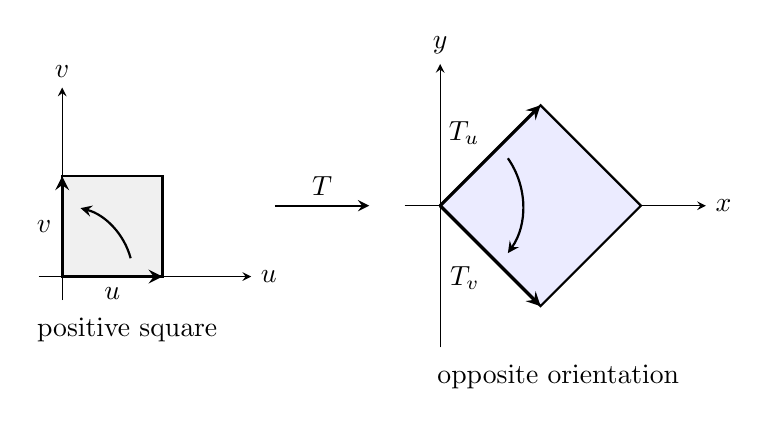
\begin{tikzpicture}[scale=0.75, >=stealth]
    \begin{scope}
        \draw[->] (-0.4,0) -- (3.2,0) node[right] {\(u\)};
        \draw[->] (0,-0.4) -- (0,3.2) node[above] {\(v\)};

        \draw[fill=gray!12, thick] (0,0) rectangle (1.7,1.7);

        \draw[->, very thick] (0,0) -- (1.7,0) node[midway, below] {\(u\)};
        \draw[->, very thick] (0,0) -- (0,1.7) node[midway, left] {\(v\)};

        % Arc perfectly centered at the origin, sweeping from u to v
        \draw[->, thick] (15:1.2) arc[start angle=15, end angle=75, radius=1.2];

        \node at (1.1,-0.9) {positive square};
    \end{scope}

    \draw[->, thick] (3.6,1.2) -- (5.2,1.2);
    \node[above] at (4.4,1.2) {\(T\)};

    \begin{scope}[shift={(6.4,1.2)}]
        \draw[->] (-0.6,0) -- (4.5,0) node[right] {\(x\)};
        \draw[->] (0,-2.4) -- (0,2.4) node[above] {\(y\)};

        \coordinate (O) at (0,0);
        \coordinate (A) at (1.7,1.7);
        \coordinate (B) at (1.7,-1.7);
        \coordinate (AB) at (3.4,0);

        \draw[fill=blue!8, thick] (O) -- (A) -- (AB) -- (B) -- cycle;

        \draw[->, very thick] (O) -- (A) node[midway, above left] {\(T_u\)};
        \draw[->, very thick] (O) -- (B) node[midway, below left] {\(T_v\)};

        % Arc perfectly centered at the origin, sweeping from T_u down to T_v
        \draw[->, thick] (35:1.4) arc[start angle=35, end angle=-35, radius=1.4];

        \node at (2,-2.9) {opposite orientation};
    \end{scope}
\end{tikzpicture}
\caption{The map \(T(u,v)=(u+v,u-v)\) sends the positive \(uv\)-orientation to the
opposite orientation in the \(xy\)-plane.}
\end{figure}

Now watch the same fact through differentials:
\[
    x=u+v,
    \qquad
    y=u-v.
\]
So
\[
    dx=du+dv,
\]
and
\[
    dy=du-dv.
\]
Therefore
\[
\begin{aligned}
dx\wedge dy
&=
(du+dv)\wedge(du-dv)\\
&=
du\wedge du-du\wedge dv+dv\wedge du-dv\wedge dv\\
&=
-du\wedge dv-du\wedge dv\\
&=
-2\,du\wedge dv.
\end{aligned}
\]
Thus
\[
\boxed{
    dx\wedge dy=-2\,du\wedge dv.
}
\]

The determinant has appeared as the coefficient of the pulled-back area form.

For ordinary area, we use the positive scale factor:
\[
    \operatorname{Area}(T(S))
    =
    \int_0^1\int_0^1 2\,du\,dv
    =
    2.
\]
For signed area using the orientation induced by the parametrization \(T\), we keep
the sign:
\[
    \int_S T^*(dx\wedge dy)
    =
    \int_0^1\int_0^1 (-2)\,du\,dv
    =
    -2.
\]

Both answers are correct.  They answer different questions.

\subsection{The determinant as the coefficient of a pulled-back area element}

The word \emph{pullback} means that we express a form from the target coordinates
back in the parameter coordinates.

If
\[
    T(u,v)=(x(u,v),y(u,v)),
\]
then pulling back \(dx\) means replacing it by the differential of \(x(u,v)\):
\[
    T^*(dx)=d(x(u,v))=x_u\,du+x_v\,dv.
\]
Similarly,
\[
    T^*(dy)=d(y(u,v))=y_u\,du+y_v\,dv.
\]

So
\[
\begin{aligned}
T^*(dx\wedge dy)
&=
(x_u\,du+x_v\,dv)\wedge(y_u\,du+y_v\,dv)\\
&=
x_u y_v\,du\wedge dv+x_v y_u\,dv\wedge du\\
&=
(x_u y_v-x_v y_u)\,du\wedge dv.
\end{aligned}
\]
Hence
\[
\boxed{
    T^*(dx\wedge dy)
    =
    \frac{\partial(x,y)}{\partial(u,v)}\,du\wedge dv.
}
\]

This is the signed version of the change-of-variables rule.

\begin{definition}[Pullback of an area form]
Let
\[
    T(u,v)=(x(u,v),y(u,v)).
\]
For a \(2\)-form
\[
    \omega=g(x,y)\,dx\wedge dy,
\]
its pullback by \(T\) is
\[
\boxed{
    T^*\omega
    =
    g(x(u,v),y(u,v))
    \frac{\partial(x,y)}{\partial(u,v)}
    \,du\wedge dv.
}
\]
\end{definition}

The pullback does two things at once:
\[
    g(x,y)\quad\longrightarrow\quad g(x(u,v),y(u,v)),
\]
and
\[
    dx\wedge dy\quad\longrightarrow\quad
    \frac{\partial(x,y)}{\partial(u,v)}\,du\wedge dv.
\]

For ordinary area integrals, the second factor becomes positive:
\[
\boxed{
    \iint_R g(x,y)\,dA
    =
    \iint_S g(T(u,v))
    \left|
    \frac{\partial(x,y)}{\partial(u,v)}
    \right|
    du\,dv.
}
\]
For oriented \(2\)-form integrals, the sign stays:
\[
\boxed{
    \iint_R g(x,y)\,dx\wedge dy
    =
    \iint_S
    g(T(u,v))
    \frac{\partial(x,y)}{\partial(u,v)}
    \,du\wedge dv,
}
\]
when \(T\) is used to orient the image.

\begin{example}[A chemical spread over a quarter disk]
A thin chemical film has areal density
\[
    g(x,y)=3+x.
\]
Let \(R\) be the quarter disk
\[
    x^2+y^2\le4,
    \qquad
    x\ge0,\qquad y\ge0.
\]
Use polar coordinates:
\[
    x=r\cos\theta,
    \qquad
    y=r\sin\theta,
\]
with
\[
    0\le r\le2,
    \qquad
    0\le\theta\le\frac{\pi}{2}.
\]

The area form pulls back as
\[
    dx\wedge dy=r\,dr\wedge d\theta.
\]
The density becomes
\[
    g(r\cos\theta,r\sin\theta)=3+r\cos\theta.
\]
So the pulled-back \(2\)-form is
\[
    (3+r\cos\theta)\,r\,dr\wedge d\theta.
\]
The total amount of chemical is
\[
\begin{aligned}
    \iint_R (3+x)\,dA
    &=
    \int_0^{\pi/2}\int_0^2
    (3+r\cos\theta)r\,dr\,d\theta\\
    &=
    \int_0^{\pi/2}
    \left[
        \frac{3r^2}{2}+\frac{r^3}{3}\cos\theta
    \right]_{0}^{2}
    d\theta\\
    &=
    \int_0^{\pi/2}
    \left(
        6+\frac83\cos\theta
    \right)d\theta\\
    &=
    3\pi+\frac83.
\end{aligned}
\]
So
\[
\boxed{
    \iint_R (3+x)\,dA=3\pi+\frac83.
}
\]
\end{example}

Here the polar Jacobian
\[
    r
\]
is nonnegative on the chosen domain, so the signed and ordinary area factors agree
except at the origin.

\subsection{Pulling back volume elements}

The same idea works in space.  Let
\[
    T(u,v,w)=(x(u,v,w),y(u,v,w),z(u,v,w)).
\]
Then
\[
    dx=x_u\,du+x_v\,dv+x_w\,dw,
\]
\[
    dy=y_u\,du+y_v\,dv+y_w\,dw,
\]
and
\[
    dz=z_u\,du+z_v\,dv+z_w\,dw.
\]
When we wedge these three expressions together, every repeated differential vanishes,
and the surviving coefficient is the \(3\times3\) determinant:
\[
\boxed{
    T^*(dx\wedge dy\wedge dz)
    =
    \frac{\partial(x,y,z)}{\partial(u,v,w)}
    \,du\wedge dv\wedge dw.
}
\]

For a \(3\)-form
\[
    \Omega=h(x,y,z)\,dx\wedge dy\wedge dz,
\]
the pullback is
\[
\boxed{
    T^*\Omega
    =
    h(T(u,v,w))
    \frac{\partial(x,y,z)}{\partial(u,v,w)}
    \,du\wedge dv\wedge dw.
}
\]

\begin{example}[A skewed box with reversed orientation]
Let
\[
    T(u,v,w)=(x,y,z)=(u+v,\;u-v,\;w).
\]
Then
\[
    dx=du+dv,
\]
\[
    dy=du-dv,
\]
and
\[
    dz=dw.
\]
Therefore
\[
\begin{aligned}
dx\wedge dy\wedge dz
&=
(du+dv)\wedge(du-dv)\wedge dw\\
&=
(-2\,du\wedge dv)\wedge dw\\
&=
-2\,du\wedge dv\wedge dw.
\end{aligned}
\]
So
\[
\boxed{
    T^*(dx\wedge dy\wedge dz)
    =
    -2\,du\wedge dv\wedge dw.
}
\]

If
\[
    S=[0,1]\times[0,1]\times[0,1],
\]
then \(T(S)\) is a skewed prism.  Its ordinary volume is
\[
    2.
\]
But its oriented volume using the parametrization \(T\) is
\[
    -2.
\]
The minus sign says that the ordered coordinate directions
\[
    T_u,\quad T_v,\quad T_w
\]
have the opposite orientation from the usual \(x,y,z\)-orientation.
\end{example}

For ordinary volume integrals, the positive rule is
\[
\boxed{
    \iiint_E h(x,y,z)\,dV
    =
    \iiint_S h(T(u,v,w))
    \left|
    \frac{\partial(x,y,z)}{\partial(u,v,w)}
    \right|
    du\,dv\,dw.
}
\]
For oriented \(3\)-form integrals, the sign stays:
\[
\boxed{
    \iiint_E h(x,y,z)\,dx\wedge dy\wedge dz
    =
    \iiint_S h(T(u,v,w))
    \frac{\partial(x,y,z)}{\partial(u,v,w)}
    \,du\wedge dv\wedge dw.
}
\]

\subsection{Orientation versus absolute value}

There are now two languages.

\[
\begin{array}{c|c|c}
\text{Object} & \text{Measures} & \text{Jacobian factor} \\ \hline
dA & \text{ordinary area} & |J|\\[1mm]
dV & \text{ordinary volume} & |J|\\[1mm]
dx\wedge dy & \text{signed area} & J\\[1mm]
dx\wedge dy\wedge dz & \text{signed volume} & J
\end{array}
\]

The ordinary symbols
\[
    dA,\qquad dV
\]
forget orientation.  They count size only.

The wedge forms
\[
    dx\wedge dy,\qquad dx\wedge dy\wedge dz
\]
remember orientation.  They count size with sign.

This is why the same determinant appears in two slightly different ways:
\[
    \text{ordinary integration uses } |J|,
\]
while
\[
    \text{oriented integration uses } J.
\]

If \(J>0\), the coordinate change preserves orientation.  If \(J<0\), it reverses
orientation.  If \(J=0\), then the derivative crushes area or volume at that point, and
the coordinate change may stop being a genuine coordinate system there.

The notation
\[
    T^*\omega
\]
is useful because it keeps the sign.  But the same sign is also where mistakes begin.
A determinant can be negative, zero, or locally correct while the map still covers the
same region more than once.  The next examples are traps worth meeting before the
formula becomes a habit.

\section{Warning examples}
\label{sec:12.6}

The determinant is a local measurement.  It knows how one tiny tile changes near one
point.  It does not know whether another tile lands on top of the same place.

That is why the change-of-variables theorem had hypotheses: smoothness, one-to-one
behavior, and nonzero Jacobian in the interior.  The examples below show what those
conditions are protecting.

\subsection{A transformation that is not one-to-one}

Polar coordinates give the cleanest warning.

Use
\[
    x=r\cos\theta,
    \qquad
    y=r\sin\theta.
\]
The Jacobian determinant is
\[
    J=r.
\]
Now choose the parameter region
\[
    S=\{(r,\theta):0\le r\le1,\ 0\le\theta\le4\pi\}.
\]
This region traces the unit disk twice.  The angles from \(0\) to \(2\pi\) cover the disk
once.  The angles from \(2\pi\) to \(4\pi\) cover it again.

If we blindly compute
\[
    \iint_S r\,dr\,d\theta,
\]
we get
\[
\begin{aligned}
    \int_0^{4\pi}\int_0^1 r\,dr\,d\theta
    &=
    \int_0^{4\pi}\frac12\,d\theta\\
    &=
    2\pi.
\end{aligned}
\]
But the ordinary area of the unit disk is
\[
    \pi.
\]
The answer is twice too large because the disk was counted twice.

\begin{figure}[h]
\centering
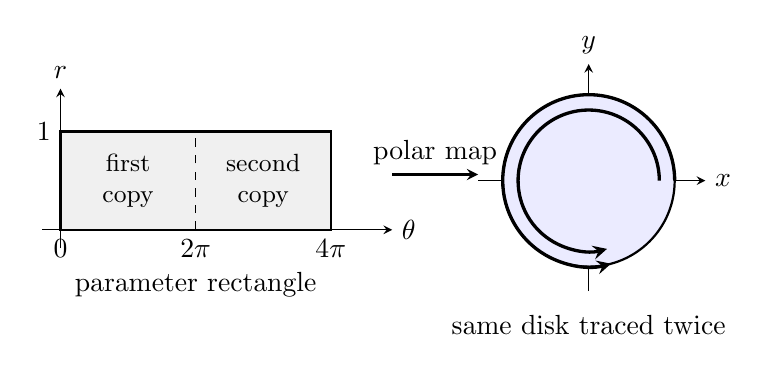
\begin{tikzpicture}[scale=0.78, >=stealth]
    \begin{scope}
        \draw[->] (-0.3,0) -- (5.4,0) node[right] {\(\theta\)};
        \draw[->] (0,-0.3) -- (0,2.3) node[above] {\(r\)};

        % Widened the rectangle slightly
        \draw[fill=gray!12, thick] (0,0) rectangle (4.4,1.6);
        \node[below] at (0,0) {\(0\)};
        \node[below] at (2.2,0) {\(2\pi\)};
        \node[below] at (4.4,0) {\(4\pi\)};
        \node[left] at (0,1.6) {\(1\)};
        \draw[dashed] (2.2,0) -- (2.2,1.6);

        \node at (2.2,-0.9) {parameter rectangle};
        
        % Stacked the text and reduced font size slightly to fit cleanly
        \node[align=center, font=\small] at (1.1,0.8) {first\\copy};
        \node[align=center, font=\small] at (3.3,0.8) {second\\copy};
    \end{scope}

    % Shifted the arrow to make room
    \draw[->, thick] (5.4,0.9) -- (6.8,0.9);
    \node[above] at (6.1,0.9) {polar map};

    % Shifted the right scope to make room
    \begin{scope}[shift={(8.6,0.8)}]
        \draw[->] (-1.8,0) -- (1.9,0) node[right] {\(x\)};
        \draw[->] (0,-1.8) -- (0,1.9) node[above] {\(y\)};

        \draw[fill=blue!8, thick] (0,0) circle (1.4);

        \draw[->, very thick] (1.4,0) arc[start angle=0,end angle=285,radius=1.4];
        \draw[->, very thick] (1.15,0) arc[start angle=0,end angle=285,radius=1.15];

        \node at (0,-2.35) {same disk traced twice};
    \end{scope}
\end{tikzpicture}
\caption{The determinant \(r\) is correct locally, but the chosen parameter region
covers the disk twice.}
\end{figure}

The formula did not fail locally.  It counted exactly what the parametrization did:
one disk with multiplicity \(2\).

For ordinary area of the image, use a one-to-one parameter region, such as
\[
    0\le r\le1,
    \qquad
    0\le\theta\le2\pi.
\]
Then
\[
    \int_0^{2\pi}\int_0^1 r\,dr\,d\theta=\pi.
\]

\subsection{A transformation with zero Jacobian at a point}

A zero Jacobian means that the derivative has crushed area or volume at that point.
Sometimes this is harmless for integration.  Polar coordinates have
\[
    J=r,
\]
which vanishes at \(r=0\), and the origin is only one point.  That single collapse does
not ruin the area formula.

But a zero Jacobian often warns us that the map is not a clean coordinate system near
that point.

Consider
\[
    T(u,v)=(x,y)=(u^2-v^2,\;2uv).
\]
This is the complex squaring map:
\[
    x+iy=(u+iv)^2.
\]
The derivative matrix is
\[
    DT(u,v)=
    \begin{pmatrix}
        2u&-2v\\
        2v&2u
    \end{pmatrix}.
\]
Its determinant is
\[
\begin{aligned}
    J_T(u,v)
    &=
    (2u)(2u)-(-2v)(2v)\\
    &=
    4u^2+4v^2\\
    &=
    4(u^2+v^2).
\end{aligned}
\]
So
\[
    J_T(0,0)=0.
\]

To see the geometry, write
\[
    u=s\cos\alpha,
    \qquad
    v=s\sin\alpha.
\]
Then
\[
\begin{aligned}
    x
    &=
    s^2\cos^2\alpha-s^2\sin^2\alpha
    =
    s^2\cos(2\alpha),
\end{aligned}
\]
and
\[
    y
    =
    2s^2\cos\alpha\sin\alpha
    =
    s^2\sin(2\alpha).
\]
So the map sends
\[
    \text{radius }s \quad\longmapsto\quad \text{radius }s^2,
\]
and
\[
    \text{angle }\alpha \quad\longmapsto\quad \text{angle }2\alpha.
\]

A tiny circle around the origin is sent to an even tinier circle, and it is traced twice.
The map folds directions together near the origin.  There is no smooth inverse
coordinate system through that point.

If \(D_a\) is the disk
\[
    u^2+v^2\le a^2,
\]
then \(T(D_a)\) is the disk
\[
    x^2+y^2\le a^4.
\]
Its ordinary area is
\[
    \pi a^4.
\]
But integrating the absolute Jacobian over the full parameter disk gives
\[
\begin{aligned}
    \iint_{D_a}4(u^2+v^2)\,du\,dv
    &=
    \int_0^{2\pi}\int_0^a 4s^2\,s\,ds\,d\alpha\\
    &=
    2\pi a^4.
\end{aligned}
\]
Again the answer is twice the image area, because the disk is covered twice.

The zero Jacobian at the origin is not the only problem.  The global problem is the
double covering.  But the zero Jacobian is a visible warning: the map is not a regular
coordinate chart at the origin.

\subsection{Why absolute value appears for ordinary area and volume}

Now take a map that is perfectly one-to-one and has nonzero determinant everywhere:
\[
    T(u,v)=(x,y)=(u,\;1-v).
\]
It sends the unit square
\[
    0\le u\le1,\qquad 0\le v\le1
\]
onto the unit square
\[
    0\le x\le1,\qquad 0\le y\le1.
\]
The image area is plainly
\[
    1.
\]

The Jacobian matrix is
\[
    DT=
    \begin{pmatrix}
        1&0\\
        0&-1
    \end{pmatrix},
\]
so
\[
    J_T=-1.
\]
If ordinary area used \(J_T\) instead of \(|J_T|\), it would give
\[
    \int_0^1\int_0^1 (-1)\,dv\,du=-1.
\]
That cannot be ordinary area.

The correct ordinary area computation is
\[
    \int_0^1\int_0^1 |{-1}|\,dv\,du=1.
\]
So the absolute value is not a technical afterthought.  It is what turns signed area
into ordinary area.

The same thing happens for volume.  The reflection
\[
    T(u,v,w)=(u,v,-w)
\]
has
\[
    J_T=-1.
\]
It preserves ordinary volume, but it reverses orientation.  So
\[
    dV=du\,dv\,dw,
\]
while
\[
    dx\wedge dy\wedge dz=-du\wedge dv\wedge dw.
\]

\subsection{Why oriented integrals remember the sign}

The sign becomes useful as soon as orientation matters.

Return to
\[
    T(u,v)=(u,1-v).
\]
Pull back the signed area form:
\[
    dx=du,
\]
and
\[
    dy=-dv.
\]
Therefore
\[
    T^*(dx\wedge dy)=du\wedge(-dv)=-du\wedge dv.
\]
So the parametrized unit square has signed area
\[
    -1.
\]

Why negative?  Follow the boundary induced by the parameter square.

The positive boundary of the \(uv\)-square goes counterclockwise:
\[
    (0,0)\to(1,0)\to(1,1)\to(0,1)\to(0,0).
\]
Under \(T\), these points become
\[
    (0,1)\to(1,1)\to(1,0)\to(0,0)\to(0,1).
\]
That path goes clockwise around the \(xy\)-square.

\begin{figure}[h]
\centering
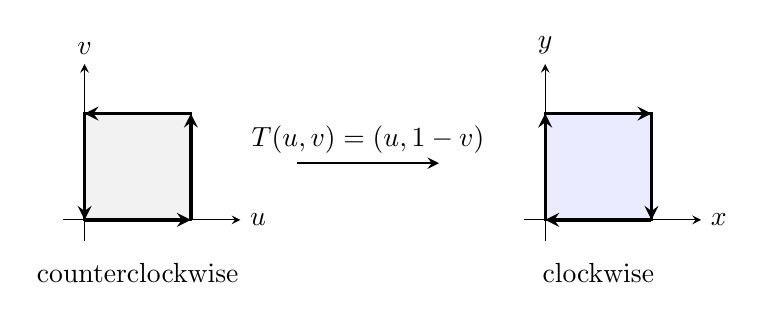
\begin{tikzpicture}[scale=0.9, >=stealth]
    \begin{scope}
        \draw[->] (-0.3,0) -- (2.2,0) node[right] {\(u\)};
        \draw[->] (0,-0.3) -- (0,2.2) node[above] {\(v\)};

        \draw[fill=gray!10, thick] (0,0) rectangle (1.5,1.5);
        \draw[->, very thick] (0,0) -- (1.5,0);
        \draw[->, very thick] (1.5,0) -- (1.5,1.5);
        \draw[->, very thick] (1.5,1.5) -- (0,1.5);
        \draw[->, very thick] (0,1.5) -- (0,0);

        \node at (0.75,-0.75) {counterclockwise};
    \end{scope}

    % Lengthened the arrow and shifted it to the right
    \draw[->, thick] (3.0,0.8) -- (5.0,0.8);
    \node[above] at (4.0,0.8) {\(T(u,v)=(u,1-v)\)};

    % Shifted the right coordinate system further out (from 5 to 6.5)
    \begin{scope}[shift={(6.5,0)}]
        \draw[->] (-0.3,0) -- (2.2,0) node[right] {\(x\)};
        \draw[->] (0,-0.3) -- (0,2.2) node[above] {\(y\)};

        \draw[fill=blue!8, thick] (0,0) rectangle (1.5,1.5);
        \draw[->, very thick] (0,1.5) -- (1.5,1.5);
        \draw[->, very thick] (1.5,1.5) -- (1.5,0);
        \draw[->, very thick] (1.5,0) -- (0,0);
        \draw[->, very thick] (0,0) -- (0,1.5);

        \node at (0.75,-0.75) {clockwise};
    \end{scope}
\end{tikzpicture}
\caption{The reflection \(y=1-v\) reverses the orientation of the square and its
boundary.}
\end{figure}

The negative sign in
\[
    T^*(dx\wedge dy)=-du\wedge dv
\]
is the same negative sign seen by walking around the boundary in the opposite
direction.

This is why oriented integrals do not use absolute value.  If we replaced \(J\) by
\[
    |J|,
\]
then clockwise and counterclockwise parametrizations would give the same answer.
That would destroy the bookkeeping needed for the theorems ahead.

The change-of-variables formula has taught us how areas and volumes transform inside
a region.  But the last example hints at another kind of transformation: the boundary
itself changes direction.  The next time orientation appears, it will be attached not to
a tiny parallelogram, but to a curve we walk along.  That is where vector fields,
work integrals, and \(1\)-forms begin.
\section{Chapter review and applications}
\label{sec:12.7}

Chapter \ref{ch:12} answered the scale-factor question left by Chapter \ref{ch:11}.
Cylindrical coordinates needed the factor
\[
    r,
\]
and spherical coordinates needed the factor
\[
    \rho^2\sin\phi.
\]
Those were not special tricks.  They were Jacobian determinants.

A change of variables has two jobs:

\[
\boxed{
\begin{array}{c}
\text{make the region simpler,}\\[1mm]
\text{and measure how the small pieces change size.}
\end{array}
}
\]

The first job is geometry.  The second job is the determinant.

\subsection{Skills: choosing and using substitutions}

A good substitution usually comes from the boundary equations.

If the boundary contains
\[
    x+y=1
    \qquad\text{and}\qquad
    x+y=4,
\]
then the expression
\[
    u=x+y
\]
is asking to become a coordinate.

If the boundary contains
\[
    xy=1
    \qquad\text{and}\qquad
    xy=5,
\]
then
\[
    u=xy
\]
may be a natural coordinate.

If the region is circular, polar coordinates are listening.  If the solid is spherical,
spherical coordinates are listening.  If the object is an ellipsoid, a stretched ball is
often hiding inside it.

\[
\begin{array}{c|c}
\text{What the geometry shows} & \text{Natural substitution} \\ \hline
\text{circles centered at the origin} & x=r\cos\theta,\ y=r\sin\theta\\[1mm]
\text{cylinders around the }z\text{-axis} & x=r\cos\theta,\ y=r\sin\theta,\ z=z\\[1mm]
\text{spheres centered at the origin} &
x=\rho\sin\phi\cos\theta,\ y=\rho\sin\phi\sin\theta,\ z=\rho\cos\phi\\[1mm]
\text{ellipses or ellipsoids} & x=au,\ y=bv,\ z=cw\\[1mm]
\text{slanted parallel lines} & u=ax+by,\ v=cx+dy\\[1mm]
\text{products and ratios} & u=xy,\ v=\dfrac{y}{x}\\[3mm]
\text{a variable ceiling }0\le z\le g(x,y) & z=g(x,y)w
\end{array}
\]

Once the substitution is chosen, the steps are always the same.

\[
\boxed{
\begin{array}{l}
\text{1. Write the map from new variables to old variables.}\\
\text{2. Translate the region.}\\
\text{3. Translate the integrand.}\\
\text{4. Compute the Jacobian determinant.}\\
\text{5. Use } |J| \text{ for ordinary area or volume.}\\
\text{6. Use } J \text{ for oriented forms.}
\end{array}
}
\]

In the plane, for
\[
    T(u,v)=(x(u,v),y(u,v)),
\]
the Jacobian determinant is
\[
\boxed{
    J_T(u,v)=
    \frac{\partial(x,y)}{\partial(u,v)}
    =
    \begin{vmatrix}
    x_u&x_v\\
    y_u&y_v
    \end{vmatrix}.
}
\]
The ordinary area rule is
\[
\boxed{
    dA=|J_T(u,v)|\,du\,dv.
}
\]
The oriented form rule is
\[
\boxed{
    T^*(dx\wedge dy)
    =
    J_T(u,v)\,du\wedge dv.
}
\]

In space, for
\[
    T(u,v,w)=(x(u,v,w),y(u,v,w),z(u,v,w)),
\]
the Jacobian determinant is
\[
\boxed{
    J_T(u,v,w)=
    \frac{\partial(x,y,z)}{\partial(u,v,w)}
    =
    \det
    \begin{pmatrix}
    x_u&x_v&x_w\\
    y_u&y_v&y_w\\
    z_u&z_v&z_w
    \end{pmatrix}.
}
\]
The ordinary volume rule is
\[
\boxed{
    dV=|J_T(u,v,w)|\,du\,dv\,dw.
}
\]
The oriented form rule is
\[
\boxed{
    T^*(dx\wedge dy\wedge dz)
    =
    J_T(u,v,w)\,du\wedge dv\wedge dw.
}
\]

The absolute value is for size.  The sign is for orientation.

\begin{figure}[h]
\centering
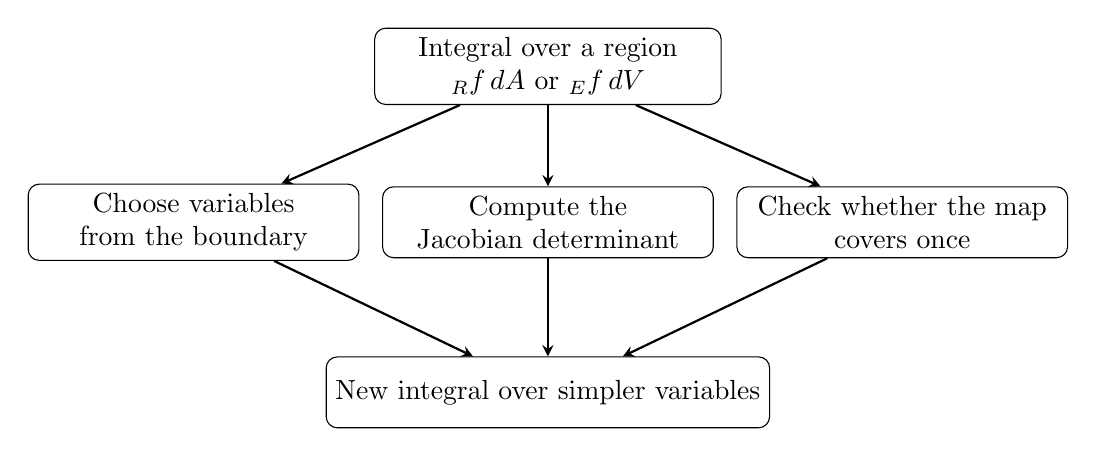
\begin{tikzpicture}[scale=0.9, >=stealth]
    \node[draw, rounded corners, align=center, minimum width=4.4cm, minimum height=0.9cm]
        (start) at (0,0) {Integral over a region\\ \(\displaystyle \iint_R f\,dA\) or \(\displaystyle \iiint_E f\,dV\)};

    \node[draw, rounded corners, align=center, minimum width=4.2cm, minimum height=0.9cm]
        (region) at (-5,-2.2) {Choose variables\\ from the boundary};

    \node[draw, rounded corners, align=center, minimum width=4.2cm, minimum height=0.9cm]
        (jac) at (0,-2.2) {Compute the\\ Jacobian determinant};

    \node[draw, rounded corners, align=center, minimum width=4.2cm, minimum height=0.9cm]
        (one) at (5,-2.2) {Check whether the map\\ covers once};

    \node[draw, rounded corners, align=center, minimum width=5.2cm, minimum height=0.9cm]
        (new) at (0,-4.6) {New integral over simpler variables};

    \draw[->, thick] (start) -- (region);
    \draw[->, thick] (start) -- (jac);
    \draw[->, thick] (start) -- (one);

    \draw[->, thick] (region) -- (new);
    \draw[->, thick] (jac) -- (new);
    \draw[->, thick] (one) -- (new);
\end{tikzpicture}
\caption{A substitution is both a geometric choice and a measurement correction.}
\end{figure}

\subsection{Worked review example: a slanted window}

A thin glass window occupies the parallelogram-like region
\[
    R=\{(x,y):1\le x+y\le3,\ 0\le x-y\le2\}.
\]
The density of tint on the glass is
\[
    q(x,y)=x+y.
\]
Find the total amount of tint:
\[
    \iint_R (x+y)\,dA.
\]

The boundary equations suggest
\[
    u=x+y,
    \qquad
    v=x-y.
\]
Then \(R\) becomes the rectangle
\[
    1\le u\le3,
    \qquad
    0\le v\le2.
\]

Solve for \(x\) and \(y\):
\[
    x=\frac{u+v}{2},
    \qquad
    y=\frac{u-v}{2}.
\]
The Jacobian determinant is
\[
\begin{aligned}
    \frac{\partial(x,y)}{\partial(u,v)}
    &=
    \det
    \begin{pmatrix}
    1/2&1/2\\
    1/2&-1/2
    \end{pmatrix}  \\
    &=
    -\frac14-\frac14\\
    &=
    -\frac12.
\end{aligned}
\]
So the ordinary area factor is
\[
    \left|
    \frac{\partial(x,y)}{\partial(u,v)}
    \right|
    =
    \frac12.
\]
The integrand becomes
\[
    x+y=u.
\]
Therefore
\[
\begin{aligned}
\iint_R (x+y)\,dA
&=
\int_1^3\int_0^2
u\cdot\frac12\,dv\,du\\
&=
\int_1^3 u\,du\\
&=
\left[\frac{u^2}{2}\right]_1^3\\
&=
4.
\end{aligned}
\]
Thus
\[
\boxed{
    \iint_R (x+y)\,dA=4.
}
\]

The signed Jacobian was negative.  That means the ordered variables \((u,v)\) reverse
the usual orientation of the \(xy\)-plane.  The glass does not have negative area, so the
ordinary integral uses the absolute value.

\subsection{Worked review example: a curved plate between hyperbolas}

A thin metal plate lies in the first quadrant.  Its edges are
\[
    xy=1,\qquad xy=4,
\]
and
\[
    \frac{y}{x}=1,\qquad \frac{y}{x}=3.
\]
Its density is
\[
    \delta(x,y)=xy.
\]
Find its mass.

The boundary equations almost name the new variables:
\[
    u=xy,
    \qquad
    v=\frac{y}{x}.
\]
Then the plate becomes the rectangle
\[
    1\le u\le4,
    \qquad
    1\le v\le3.
\]

Because we are in the first quadrant, \(x>0\) and \(y>0\).  From
\[
    u=xy,
    \qquad
    v=\frac{y}{x},
\]
we get
\[
    y=vx.
\]
Then
\[
    u=x(vx)=vx^2,
\]
so
\[
    x=\sqrt{\frac{u}{v}}.
\]
Also,
\[
    y=vx=\sqrt{uv}.
\]
Thus
\[
    x=\sqrt{\frac{u}{v}},
    \qquad
    y=\sqrt{uv}.
\]

Compute the Jacobian.  A quick way is to compute the determinant of the forward map
\[
    (x,y)\longmapsto (u,v).
\]
Since
\[
    u=xy,
    \qquad
    v=\frac{y}{x},
\]
we have
\[
    \frac{\partial(u,v)}{\partial(x,y)}
    =
    \det
    \begin{pmatrix}
    y&x\\[1mm]
    -y/x^2&1/x
    \end{pmatrix}.
\]
Therefore
\[
\begin{aligned}
    \frac{\partial(u,v)}{\partial(x,y)}
    &=
    y\cdot\frac1x
    -
    x\left(-\frac{y}{x^2}\right)\\
    &=
    \frac{y}{x}+\frac{y}{x}\\
    &=
    2\frac{y}{x}\\
    &=
    2v.
\end{aligned}
\]
So
\[
\boxed{
    \frac{\partial(x,y)}{\partial(u,v)}=\frac{1}{2v}.
}
\]
The density becomes
\[
    \delta(x,y)=xy=u.
\]
Thus
\[
\begin{aligned}
M
&=
\iint_R xy\,dA\\
&=
\int_1^4\int_1^3
u\cdot\frac{1}{2v}\,dv\,du\\
&=
\frac12
\left(\int_1^4 u\,du\right)
\left(\int_1^3 \frac{1}{v}\,dv\right)\\
&=
\frac12
\left[\frac{u^2}{2}\right]_1^4
\left[\ln v\right]_1^3\\
&=
\frac12\cdot\frac{15}{2}\cdot\ln 3\\
&=
\frac{15}{4}\ln 3.
\end{aligned}
\]
So
\[
\boxed{
    M=\frac{15}{4}\ln 3.
}
\]

The region looked awkward in \(x,y\).  It was a rectangle in the variables its own
edges were already using.

\subsection{Worked review example: a stretched ball}

Let \(E\) be the ellipsoid
\[
    \frac{x^2}{4}+\frac{y^2}{9}+z^2\le1.
\]
Its density is
\[
    \delta(x,y,z)=
    1+\frac{x^2}{4}+\frac{y^2}{9}+z^2.
\]
Find the mass.

The ellipsoid is a stretched unit ball.  Use
\[
    x=2u,
    \qquad
    y=3v,
    \qquad
    z=w.
\]
Then
\[
    \frac{x^2}{4}+\frac{y^2}{9}+z^2
    =
    u^2+v^2+w^2.
\]
So the solid \(E\) becomes the unit ball
\[
    B=\{(u,v,w):u^2+v^2+w^2\le1\}.
\]

The Jacobian determinant is
\[
    \det
    \begin{pmatrix}
    2&0&0\\
    0&3&0\\
    0&0&1
    \end{pmatrix}
    =
    6.
\]
The density becomes
\[
    \delta=1+u^2+v^2+w^2.
\]
Therefore
\[
\begin{aligned}
M
&=
\iiint_E
\left(
1+\frac{x^2}{4}+\frac{y^2}{9}+z^2
\right)dV\\
&=
\iiint_B
6(1+u^2+v^2+w^2)\,du\,dv\,dw.
\end{aligned}
\]
Now use spherical coordinates in the \(uvw\)-space:
\[
    u^2+v^2+w^2=\rho^2,
    \qquad
    dV_{uvw}=\rho^2\sin\phi\,d\rho\,d\phi\,d\theta.
\]
The unit ball is
\[
    0\le\rho\le1,
    \qquad
    0\le\phi\le\pi,
    \qquad
    0\le\theta\le2\pi.
\]
Thus
\[
\begin{aligned}
M
&=
6\int_0^{2\pi}\int_0^\pi\int_0^1
(1+\rho^2)\rho^2\sin\phi\,d\rho\,d\phi\,d\theta\\
&=
6
\left(\int_0^{2\pi}d\theta\right)
\left(\int_0^\pi \sin\phi\,d\phi\right)
\left(\int_0^1(\rho^2+\rho^4)\,d\rho\right)\\
&=
6(2\pi)(2)
\left(\frac13+\frac15\right)\\
&=
24\pi\cdot\frac{8}{15}\\
&=
\frac{64\pi}{5}.
\end{aligned}
\]
So
\[
\boxed{
    M=\frac{64\pi}{5}.
}
\]

Two coordinate changes worked together.  The first turned the ellipsoid into a ball.
The second used spherical coordinates because the new ball had radial symmetry.

\subsection{Concept check}

\begin{enumerate}
\item What does the Jacobian determinant measure geometrically in a plane change of
variables?

\item What does the Jacobian determinant measure geometrically in a space change of
variables?

\item Why does an ordinary area or volume integral use
\[
    |J|
\]
instead of \(J\)?

\item What information is kept by
\[
    dx\wedge dy
\]
but forgotten by
\[
    dA?
\]

\item What information is kept by
\[
    dx\wedge dy\wedge dz
\]
but forgotten by
\[
    dV?
\]

\item In the plane, why does
\[
    T^*(dx\wedge dy)
    =
    \frac{\partial(x,y)}{\partial(u,v)}\,du\wedge dv
\]
contain the signed Jacobian, not its absolute value?

\item Why must a change of variables be one-to-one on the interior of the parameter
region?

\item Why are boundary overlaps usually harmless?

\item Why does polar coordinates having \(J=r=0\) at \(r=0\) not ruin the area formula
for a disk?

\item What goes wrong if a transformation has \(J=0\) on a whole two-dimensional or
three-dimensional patch?

\item Why should a map with a crease be split into smooth pieces before applying the
change-of-variables theorem?

\item What does it mean to say that polar coordinates with
\[
    0\le\theta\le4\pi
\]
cover a disk with multiplicity \(2\)?

\item How can the equations of a region's boundary suggest useful new variables?

\item What is the difference between changing the integrand and changing the area or
volume element?

\item Why is the determinant rule a local rule, while the one-to-one condition is a global
condition?
\end{enumerate}

\subsection{Skill problems}

\begin{enumerate}
\item For
\[
    x=3u-v,
    \qquad
    y=u+2v,
\]
compute
\[
    \frac{\partial(x,y)}{\partial(u,v)}.
\]

\item Let \(S\) be the unit square
\[
    0\le u\le1,\qquad 0\le v\le1.
\]
Under
\[
    x=3u-v,
    \qquad
    y=u+2v,
\]
find the area of \(T(S)\).

\item Let \(R\) be the image of the unit square under
\[
    x=2u+v,
    \qquad
    y=u+4v.
\]
Compute
\[
    \iint_R (x-y)\,dA.
\]

\item Let
\[
    u=x+y,
    \qquad
    v=x-y.
\]
Find \(x\) and \(y\) in terms of \(u\) and \(v\), and compute
\[
    \frac{\partial(x,y)}{\partial(u,v)}.
\]

\item Let
\[
    R=\{(x,y):0\le x+y\le2,\ 1\le x-y\le3\}.
\]
Use
\[
    u=x+y,
    \qquad
    v=x-y
\]
to find the area of \(R\).

\item Use polar coordinates to compute the area of the disk
\[
    x^2+y^2\le a^2.
\]

\item Use polar coordinates to compute
\[
    \iint_R (x^2+y^2)\,dA,
\]
where \(R\) is the annulus
\[
    1\le x^2+y^2\le4.
\]

\item A thin circular plate has radius \(3\) and density
\[
    \delta(x,y)=5-x^2-y^2.
\]
Use polar coordinates to find its mass.

\item Let \(R\) be the first-quadrant region bounded by
\[
    xy=2,\qquad xy=6,
\]
and
\[
    \frac{y}{x}=1,\qquad \frac{y}{x}=4.
\]
Use
\[
    u=xy,
    \qquad
    v=\frac{y}{x}
\]
to find the area of \(R\).

\item For the same region as Problem 9, compute
\[
    \iint_R xy\,dA.
\]

\item Let
\[
    T(u,v)=(u^2-v^2,\ 2uv).
\]
Compute
\[
    T^*(dx\wedge dy).
\]
Where does the Jacobian vanish?

\item Explain why the map
\[
    T(u,v)=(u^2-v^2,\ 2uv)
\]
covers most of its image twice if the domain is a disk centered at the origin.

\item Let
\[
    T(u,v)=(u,\ 1-v).
\]
Compute
\[
    T^*(dx\wedge dy).
\]
Does this map preserve or reverse orientation?

\item Let
\[
    T(u,v,w)=(2u,\ 3v,\ 4w).
\]
Find the volume scale factor.

\item Use the substitution
\[
    x=2u,\qquad y=3v,\qquad z=4w
\]
to find the volume of the ellipsoid
\[
    \frac{x^2}{4}+\frac{y^2}{9}+\frac{z^2}{16}\le1.
\]

\item Use cylindrical coordinates to compute the volume of the solid cylinder
\[
    x^2+y^2\le9,
    \qquad
    0\le z\le5.
\]

\item Use spherical coordinates to compute the volume of the ball
\[
    x^2+y^2+z^2\le a^2.
\]

\item A ball of radius \(2\) has density
\[
    \delta(\rho)=4-\rho.
\]
Use spherical coordinates to find its mass.

\item Let
\[
    T(u,v,w)=(u,\ v,\ uvw).
\]
Compute the Jacobian determinant.

\item Use
\[
    x=u,\qquad y=v,\qquad z=u(1+v)w
\]
to find the volume of
\[
    E=\{(x,y,z):1\le x\le2,\ 0\le y\le1,\ 0\le z\le x(1+y)\}.
\]

\item Let
\[
    x=r\cos\theta,
    \qquad
    y=r\sin\theta.
\]
Compute
\[
    dx\wedge dy
\]
in terms of \(dr\) and \(d\theta\).

\item Let
\[
    x=r\cos\theta,
    \qquad
    y=r\sin\theta,
    \qquad
    z=z.
\]
Compute
\[
    dx\wedge dy\wedge dz
\]
in terms of \(dr,d\theta,dz\).

\item Let
\[
    x=\rho\sin\phi\cos\theta,
    \quad
    y=\rho\sin\phi\sin\theta,
    \quad
    z=\rho\cos\phi.
\]
State the volume element in spherical coordinates.

\item Decide whether the following parameter region covers its image once, twice, or with
boundary overlap only:
\[
    0\le r\le2,\qquad 0\le\theta\le2\pi.
\]
Explain.

\item Decide whether the following parameter region covers its image once, twice, or with
boundary overlap only:
\[
    0\le r\le2,\qquad 0\le\theta\le4\pi.
\]
Explain.

\item Choose useful variables for the region bounded by
\[
    y=2x,\qquad y=5x,\qquad x^2+y^2=1,\qquad x^2+y^2=9.
\]
Do not evaluate an integral.  Just explain the substitution.

\item Choose useful variables for the region bounded by
\[
    x+y=1,\qquad x+y=4,\qquad x-2y=0,\qquad x-2y=3.
\]
Do not evaluate an integral.  Just explain the substitution.

\item Write the ordinary and oriented change-of-variables rules for a plane transformation.

\item Write the ordinary and oriented change-of-variables rules for a space transformation.

\item Give an example of a transformation whose Jacobian is correct locally but whose
parameter region covers the same image twice.
\end{enumerate}

\subsection{Project: Gaussian integrals and polar coordinates}

The integral
\[
    \int e^{-x^2}\,dx
\]
has no elementary antiderivative.  That is a single-variable problem.  The surprising
way through it is to square the integral and make it two-dimensional.

Let
\[
    I=\int_{-\infty}^{\infty}e^{-x^2}\,dx.
\]
This integral is positive, so if we can find \(I^2\), then we can find \(I\).

\subsubsection*{Part 1. Square the integral}

Write
\[
\begin{aligned}
I^2
&=
\left(\int_{-\infty}^{\infty}e^{-x^2}\,dx\right)
\left(\int_{-\infty}^{\infty}e^{-y^2}\,dy\right).
\end{aligned}
\]
The second variable is called \(y\) so the two copies can be combined as a double
integral:
\[
\boxed{
I^2
=
\iint_{\mathbb R^2} e^{-(x^2+y^2)}\,dA.
}
\]
The integrand is now radial:
\[
    e^{-(x^2+y^2)}=e^{-r^2}.
\]
The region is the whole plane.  Polar coordinates fit both the integrand and the region.

\subsubsection*{Part 2. Change to polar coordinates}

In polar coordinates,
\[
    dA=r\,dr\,d\theta.
\]
Therefore
\[
\begin{aligned}
I^2
&=
\int_0^{2\pi}\int_0^\infty e^{-r^2}r\,dr\,d\theta.
\end{aligned}
\]
The inner integral uses the substitution
\[
    s=r^2,
    \qquad
    ds=2r\,dr.
\]
So
\[
\begin{aligned}
\int_0^\infty e^{-r^2}r\,dr
&=
\frac12\int_0^\infty e^{-s}\,ds\\
&=
\frac12.
\end{aligned}
\]
Thus
\[
\begin{aligned}
I^2
&=
\int_0^{2\pi}\frac12\,d\theta\\
&=
\pi.
\end{aligned}
\]
Since \(I>0\),
\[
\boxed{
    \int_{-\infty}^{\infty}e^{-x^2}\,dx=\sqrt{\pi}.
}
\]

This is one of the most famous uses of polar coordinates.  A one-variable antiderivative
was unavailable, but a two-dimensional symmetry solved the definite integral.

\subsubsection*{Part 3. A careful finite-radius version}

For a radius \(R>0\), define
\[
    G(R)=\iint_{x^2+y^2\le R^2} e^{-(x^2+y^2)}\,dA.
\]
Use polar coordinates:
\[
\begin{aligned}
G(R)
&=
\int_0^{2\pi}\int_0^R e^{-r^2}r\,dr\,d\theta\\
&=
2\pi\left[-\frac12e^{-r^2}\right]_0^R\\
&=
\pi(1-e^{-R^2}).
\end{aligned}
\]
So
\[
\boxed{
    G(R)=\pi(1-e^{-R^2}).
}
\]
As \(R\to\infty\),
\[
    G(R)\to\pi.
\]
That is the polar-coordinate shadow of
\[
    I^2=\pi.
\]

\subsubsection*{Part 4. A scaled Gaussian}

Let \(a>0\).  Find
\[
    I(a)=\int_{-\infty}^{\infty}e^{-ax^2}\,dx.
\]
Use the substitution
\[
    u=\sqrt a\,x.
\]
Then
\[
    dx=\frac{1}{\sqrt a}\,du,
\]
and
\[
\begin{aligned}
I(a)
&=
\int_{-\infty}^{\infty}e^{-u^2}\frac{1}{\sqrt a}\,du\\
&=
\frac{1}{\sqrt a}\sqrt\pi.
\end{aligned}
\]
Thus
\[
\boxed{
    \int_{-\infty}^{\infty}e^{-ax^2}\,dx
    =
    \sqrt{\frac{\pi}{a}}.
}
\]

\subsubsection*{Part 5. Normalizing the normal density}

A probability density on the real line must integrate to \(1\).  The bell-shaped density
with mean \(0\) and spread parameter \(\sigma>0\) has the form
\[
    p(x)=C e^{-x^2/(2\sigma^2)}.
\]
Find \(C\).

Using the scaled Gaussian formula with
\[
    a=\frac{1}{2\sigma^2},
\]
we get
\[
\int_{-\infty}^{\infty}e^{-x^2/(2\sigma^2)}\,dx
=
\sqrt{2\pi\sigma^2}
=
\sigma\sqrt{2\pi}.
\]
Therefore
\[
    1=C\sigma\sqrt{2\pi},
\]
so
\[
\boxed{
    C=\frac{1}{\sigma\sqrt{2\pi}}.
}
\]
Thus the normalized density is
\[
\boxed{
    p(x)=\frac{1}{\sigma\sqrt{2\pi}}e^{-x^2/(2\sigma^2)}.
}
\]

\subsubsection*{What to hand in}

Write a short report with the following pieces.

\begin{enumerate}
\item Explain why the single-variable antiderivative is not the point of this problem.

\item Show how squaring the integral produces a double integral over \(\mathbb R^2\).

\item Evaluate the double integral using polar coordinates.

\item Compute
\[
    \int_{-\infty}^{\infty} e^{-ax^2}\,dx
\]
for \(a>0\).

\item Use the result to find the normalizing constant for
\[
    C e^{-x^2/(2\sigma^2)}.
\]

\item Write one paragraph explaining why polar coordinates were the right coordinates for
the squared integral.
\end{enumerate}

The last paragraph is the heart of the project.  The formula
\[
    e^{-x^2}
\]
does not look circular.  But after squaring the integral, the expression
\[
    e^{-(x^2+y^2)}
\]
reveals a hidden disk symmetry.

\subsection{Hook: the boundary of a region now begins to matter}

Change of variables taught us to respect the inside of a region.  Tiny squares became
parallelograms.  Tiny boxes became parallelepipeds.  The determinant kept track of
how much size changed, and the wedge product kept track of orientation.

But the warning examples kept pointing toward the boundary.  A square reflected by
\[
    (u,v)\mapsto (u,1-v)
\]
did not change its ordinary area, but it reversed the direction in which its boundary was
walked.  A polar rectangle with
\[
    0\le\theta\le4\pi
\]
did not describe a larger disk; it walked around the same disk twice.

So far, the boundary has mostly helped us write bounds.  Soon it will become an object
we integrate over.  A force field can do work along a path.  A swirling fluid can have
circulation around a closed curve.  A \(1\)-form
\[
    P\,dx+Q\,dy+R\,dz
\]
is built to be added along such a path.

The question waiting for us is no longer only
\[
    \text{How much is spread through a region?}
\]
It is also
\[
    \text{What happens as we walk along its edge?}
\]
That edge question begins the next part of the book.
